%===============================================================================
% LaTeX sjabloon voor de bachelorproef toegepaste informatica aan HOGENT
% Meer info op https://github.com/HoGentTIN/latex-hogent-report
%===============================================================================

\documentclass[dutch,dit,thesis]{hogentreport}

% TODO:
% - If necessary, replace the option `dit`' with your own department!
%   Valid entries are dbo, dbt, dgz, dit, dlo, dog, dsa, soa
% - If you write your thesis in English (remark: only possible after getting
%   explicit approval!), remove the option "dutch," or replace with "english".

\usepackage{lipsum} % For blind text, can be removed after adding actual content

%% Pictures to include in the text can be put in the graphics/ folder
\graphicspath{{../graphics/}}

%% For source code highlighting, requires pygments to be installed
%% Compile with the -shell-escape flag!
%% \usepackage[chapter]{minted}
%% If you compile with the make_thesis.{bat,sh} script, use the following
%% import instead:
%%\usepackage[chapter,outputdir=../output]{minted}
\usepackage[chapter]{minted}
\usemintedstyle{solarized-light}




%% Formatting for minted environments.
\setminted{%
    autogobble,
    frame=lines,
    breaklines,
    linenos,
    tabsize=4
}

%% Ensure the list of listings is in the table of contents
\renewcommand\listoflistingscaption{%
    \IfLanguageName{dutch}{Lijst van codefragmenten}{List of listings}
}
\renewcommand\listingscaption{%
    \IfLanguageName{dutch}{Codefragment}{Listing}
}
\renewcommand*\listoflistings{%
    \cleardoublepage\phantomsection\addcontentsline{toc}{chapter}{\listoflistingscaption}%
    \listof{listing}{\listoflistingscaption}%
}

% Other packages not already included can be imported here

%%---------- Document metadata -------------------------------------------------
% TODO: Replace this with your own information
\author{Victor De Clercq}
\supervisor{Gilles Blondeel}
\cosupervisor{Elias De Smett}
\title[]%
    {Verbetering van de nauwkeurigheid van salesvoorspellingen door klantcategorieën op basis van aankoopgedrag}
\academicyear{\advance\year by -1 \the\year--\advance\year by 1 \the\year}
\examperiod{1}
\degreesought{\IfLanguageName{dutch}{Professionele bachelor in de toegepaste informatica}{Bachelor of applied computer science}}
\partialthesis{false} %% To display 'in partial fulfilment'
%\institution{Internshipcompany BVBA.}

%% Add global exceptions to the hyphenation here
\hyphenation{back-slash}

%% The bibliography (style and settings are  found in hogentthesis.cls)
\addbibresource{bachproef.bib}            %% Bibliography file
\addbibresource{../voorstel/voorstel.bib} %% Bibliography research proposal
\defbibheading{bibempty}{}

%% Prevent empty pages for right-handed chapter starts in twoside mode
\renewcommand{\cleardoublepage}{\clearpage}

\renewcommand{\arraystretch}{1.2}

%% Content starts here.
\begin{document}

%---------- Front matter -------------------------------------------------------

\frontmatter

\hypersetup{pageanchor=false} %% Disable page numbering references
%% Render a Dutch outer title page if the main language is English
\IfLanguageName{english}{%
    %% If necessary, information can be changed here
    \degreesought{Professionele Bachelor toegepaste informatica}%
    \begin{otherlanguage}{dutch}%
       \maketitle%
    \end{otherlanguage}%
}{}

%% Generates title page content
\maketitle
\hypersetup{pageanchor=true}

%%=============================================================================
%% Voorwoord
%%=============================================================================

\chapter*{\IfLanguageName{dutch}{Woord vooraf}{Preface}}%
\label{ch:voorwoord}

%% TODO:
%% Het voorwoord is het enige deel van de bachelorproef waar je vanuit je
%% eigen standpunt (``ik-vorm'') mag schrijven. Je kan hier bv. motiveren
%% waarom jij het onderwerp wil bespreken.
%% Vergeet ook niet te bedanken wie je geholpen/gesteund/... heeft

Het schrijven van deze bachelorproef markeert het einde van mijn opleiding Toegepaste Informatica aan de Hogeschool Gent. Deze periode was gevuld met leerkansen, uitdagingen en persoonlijke groei. Gedurende deze opleiding heb ik niet alleen mijn kennis in informatica verdiept, maar ook geleerd hoe ik deze kon toepassen in de realiteit.

\vspace{1em}

Deze bachelorproef kwam tot stand vanuit mijn interesse in data en AI en hoe dit op een slimme manier gebruikt kan worden. Ik onderzocht of klantsegmentatie kan helpen om verkoopvoorspellingen nauwkeuriger te maken met behulp van regressiemodellen.

\vspace{1em}

Graag wil ik mijn promotor Gilles Blondeel bedanken voor zijn begeleiding en waardevolle feedback gedurende de bachelorproef. Mijn co-promotor Elias De Smett ben ik bijzonder dankbaar voor zijn praktische ondersteuning en hulp bij de technische uitwerking van de proof-of-concept. Tot slot wil ik mijn stagementor, Mathieu Goossens, bedanken voor zijn begeleiding en de waardevolle inzichten die ik heb opgedaan tijdens het uitvoeren van mijn bachelorproef bij IPCOM NV.

\vspace{1em}

Daarnaast ben ik mijn vrienden en familie erg dankbaar voor hun voortdurende ondersteuning en aanmoediging. Hun aanwezigheid en geloof in mij hebben me keer op keer de moed gegeven om vooruit te blijven gaan.



%%=============================================================================
%% Samenvatting
%%=============================================================================

% TODO: De "abstract" of samenvatting is een kernachtige (~ 1 blz. voor een
% thesis) synthese van het document.
%
% Een goede abstract biedt een kernachtig antwoord op volgende vragen:
%
% 1. Waarover gaat de bachelorproef?
% 2. Waarom heb je er over geschreven?
% 3. Hoe heb je het onderzoek uitgevoerd?
% 4. Wat waren de resultaten? Wat blijkt uit je onderzoek?
% 5. Wat betekenen je resultaten? Wat is de relevantie voor het werkveld?
%
% Daarom bestaat een abstract uit volgende componenten:
%
% - inleiding + kaderen thema
% - probleemstelling
% - (centrale) onderzoeksvraag
% - onderzoeksdoelstelling
% - methodologie
% - resultaten (beperk tot de belangrijkste, relevant voor de onderzoeksvraag)
% - conclusies, aanbevelingen, beperkingen
%
% LET OP! Een samenvatting is GEEN voorwoord!

%%---------- Nederlandse samenvatting -----------------------------------------
%
% TODO: Als je je bachelorproef in het Engels schrijft, moet je eerst een
% Nederlandse samenvatting invoegen. Haal daarvoor onderstaande code uit
% commentaar.
% Wie zijn bachelorproef in het Nederlands schrijft, kan dit negeren, de inhoud
% wordt niet in het document ingevoegd.

\IfLanguageName{english}{%
\selectlanguage{dutch}
\chapter*{Samenvatting}

\selectlanguage{english}
}{}

%%---------- Samenvatting -----------------------------------------------------
% De samenvatting in de hoofdtaal van het document
 
\chapter*{\IfLanguageName{dutch}{Samenvatting}{Abstract}}


Dit onderzoek gaat na of het gebruik van klantsegmentatie op basis van hun koopgedrag de nauwkeurigheid van een regressievoorspellingsmodel kan verbeteren. Door klanten in verschillende groepen in te delen op basis van hun aankoopgedrag, kan een model beter rekening houden met specifieke patronen en variaties binnen de dataset en nauwkeurigere voorspellingen maken.

\vspace{1em} 

Een uitgebreid plan werd uitgevoerd, waarbij de resultaten werden geanalyseerd voor IPCOM NV, met specifieke focus op het dochterbedrijf ISOPARTNER NL, waar de data werd verzameld. Dit onderzoek werd uitgevoerd met de Microsoft Fabric-omgeving, waarbij specifiek gebruik werd gemaakt van Dataflows Gen2 voor het voorbereiden en opschonen van de data, Lakehouses voor de opslag ervan, en Machine Learning-notebooks voor de laatste schoonmaakstappen, het trainen en toepassen van het model.

\vspace{1em}

Binnen deze omgeving werd historische verkoopdata op artikelniveau verzameld en geanalyseerd om klanten te groeperen op basis van hun aankoopgedrag, zoals patronen in hun uitgaven, aankoopfrequentie en productvoorkeuren, met behulp van segmentatiemodellen. Vervolgens werd dit gebruikt in regressiemodellen om te bepalen of de voorspellingen nauwkeuriger werden door klantsegmentatie. De regressiemodellen werden afzonderlijk voor elk klantsegment toegepast, zodat er voor elk segment een specifieke voorspelling werd gemaakt.

\vspace{1em}

De resultaten zijn beoordeeld op basis van nauwkeurigheid van het model en dit werd gemeten door verschillende maatstaven zoals de Mean Absolute Error (MAE), Root Mean Squared Error (RMSE) en  Mean Squared Error (MSE). Uit de resultaten van het onderzoek blijkt dat de klantsegmentatie effectief een positieve bijdrage heeft aan de precisie van de voorspellingen met behulp van een regressie model. Dit onderzoek biedt inzicht in hoe klantendata effectief kan worden ingezet voor verdere optimalisaties binnen de Machine Learning-tools van Microsoft Fabric.



%---------- Inhoud, lijst figuren, ... -----------------------------------------

\tableofcontents

% In a list of figures, the complete caption will be included. To prevent this,
% ALWAYS add a short description in the caption!
%
%  \caption[short description]{elaborate description}
%
% If you do, only the short description will be used in the list of figures

\listoffigures

% If you included tables and/or source code listings, uncomment the appropriate
% lines.
\listoftables

\listoflistings

% Als je een lijst van afkortingen of termen wil toevoegen, dan hoort die
% hier thuis. Gebruik bijvoorbeeld de ``glossaries'' package.
% https://www.overleaf.com/learn/latex/Glossaries

%---------- Kern ---------------------------------------------------------------

\mainmatter{}

% De eerste hoofdstukken van een bachelorproef zijn meestal een inleiding op
% het onderwerp, literatuurstudie en verantwoording methodologie.
% Aarzel niet om een meer beschrijvende titel aan deze hoofdstukken te geven of
% om bijvoorbeeld de inleiding en/of stand van zaken over meerdere hoofdstukken
% te verspreiden!

%%=============================================================================
%% Inleiding
%%=============================================================================

\chapter{\IfLanguageName{dutch}{Inleiding}{Introduction}}%
\label{ch:inleiding}


\section{\IfLanguageName{dutch}{Probleemstelling}{Problem Statement}}%
\label{sec:probleemstelling}

Het voorspellen van sales en winst is een essentieel proces voor elk bedrijf dat strategische beslissingen wil nemen of financiële plannen wil opstellen. In de huidige tijd is het bijna onmogelijk om dit effectief te doen zonder gebruik te maken van data-analyse en andere technieken zoals klantsegmentatie. Bedrijven worden geconfronteerd met een steeds dynamischere markt, wat ervoor zorgt dat traditionele voorspellingsmethoden vaak tekortschieten.
 
\vspace{1em}

De doelgroep van dit onderzoek richt zich specifiek op managers en analisten in commerciële en financiële functies binnen bedrijven. Commercieel managers zijn verantwoordelijk voor het optimaliseren van verkoopstrategieën, terwijl financiële analisten gefocust zijn op het opstellen van nauwkeurige budgetten. Beide rollen zijn direct afhankelijk van betrouwbare en data gedreven voorspellingen om strategische beslissingen te ondersteunen.

\vspace{55mm}

\section{\IfLanguageName{dutch}{Onderzoeksvraag}{Research question}}%
\label{sec:onderzoeksvraag}

De centrale onderzoeksvraag van deze studie luidt: \textit{Kan klantsegmentatie op basis van aankoopgedrag de nauwkeurigheid van salesvoorspellingen verbeteren?}

Om deze vraag te beantwoorden, worden de volgende deelvragen onderzocht:

\begin{itemize}
    \item Wat is efficiënter bij het voorspellen van sales, forecastmethoden zoals SARIMA of regressiemodellen?
    \item Welke regressiemodellen presteren het best bij het voorspellen van sales?
     \item Welke clusteringtechnieken, zoals K-means, GMM, DBSCAN en K-Modes, leveren de meest betekenisvolle klantsegmenten op voor het verbeteren van salesvoorspellingen?
    \item Welke regressiemodellen presteren het best bij het voorspellen van sales in combinatie met een klantsegmentatie?
    \item Hoe kan klantsegmentatie effectief worden geïntegreerd in een regressiemodel voor salesvoorspellingen om de nauwkeurigheid te verbeteren?
\end{itemize}



\section{\IfLanguageName{dutch}{Onderzoeksdoelstelling}{Research objective}}%
\label{sec:onderzoeksdoelstelling}

Het eindresultaat van dit onderzoek is een proof-of-concept voor het bedrijf IPCOM NV, waarbij de nauwkeurigheid van salesvoorspellingen met en zonder klantsegmentatie wordt vergeleken. Het succes van deze bachelorproef wordt bepaald door het aantonen dat klantsegmentatie de precisie van de voorspellingen verbetert, gemeten aan de hand van maatstaven zoals Mean Squared Error (MSE), Mean Absolute Error (MAE) en Root Mean Squared Error (RMSE)."

\section{\IfLanguageName{dutch}{Opzet van deze bachelorproef}{Structure of this bachelor thesis}}%
\label{sec:opzet-bachelorproef}

De rest van deze bachelorproef is als volgt opgebouwd:

In Hoofdstuk~\ref{ch:stand-van-zaken} wordt een overzicht gegeven van de stand van zaken binnen het onderzoeksdomein, op basis van een literatuurstudie.

In Hoofdstuk~\ref{ch:methodologie} wordt de methodologie toegelicht en worden de gebruikte onderzoekstechnieken besproken om een antwoord te kunnen formuleren op de onderzoeksvragen.

In Hoofdstuk~\ref{ch:Proof of concept} wordt een proof of concept uitgewerkt en worden de deelvragen en de hoofdvraag aan de hand daarvan beantwoord.

In Hoofdstuk~\ref{ch:conclusie}, tenslotte, wordt de conclusie gegeven en een antwoord geformuleerd op de onderzoeksvragen. Daarbij wordt ook een aanzet gegeven voor toekomstig onderzoek binnen dit domein
\chapter{\IfLanguageName{dutch}{Stand van zaken}{State of the art}}%
\label{ch:stand-van-zaken}


% Tip: Begin elk hoofdstuk met een paragraaf inleiding die beschrijft hoe
% dit hoofdstuk past binnen het geheel van de bachelorproef. Geef in het
% bijzonder aan wat de link is met het vorige en volgende hoofdstuk.

% Pas na deze inleidende paragraaf komt de eerste sectiehoofding.

%Dit hoofdstuk bevat je literatuurstudie. De inhoud gaat verder op de inleiding, maar zal het onderwerp van de bachelorproef *diepgaand* uitspitten. De bedoeling is dat de lezer na lezing van dit hoofdstuk helemaal op de hoogte is van de huidige stand van zaken (state-of-the-art) in het onderzoeksdomein. Iemand die niet vertrouwd is met het onderwerp, weet nu voldoende om de rest van het verhaal te kunnen volgen, zonder dat die er nog andere informatie moet over opzoeken \autocite{Pollefliet2011}.

%Je verwijst bij elke bewering die je doet, vakterm die je introduceert, enz.\ naar je bronnen. In \LaTeX{} kan dat met het commando \texttt{$\backslash${textcite\{\}}} of \texttt{$\backslash${autocite\{\}}}. Als argument van het commando geef je de ``sleutel'' van een ``record'' in een bibliografische databank in het Bib\LaTeX{}-formaat (een tekstbestand). Als je expliciet naar de auteur verwijst in de zin (narratieve referentie), gebruik je \texttt{$\backslash${}textcite\{\}}. Soms is de auteursnaam niet expliciet een onderdeel van de zin, dan gebruik je \texttt{$\backslash${}autocite\{\}} (referentie tussen haakjes). Dit gebruik je bv.~bij een citaat, of om in het bijschrift van een overgenomen afbeelding, broncode, tabel, enz. te verwijzen naar de bron. In de volgende paragraaf een voorbeeld van elk.

%\textcite{Knuth1998} schreef een van de standaardwerken over sorteer- en zoekalgoritmen. Experten zijn het erover eens dat cloud computing een interessante opportuniteit vormen, zowel voor gebruikers als voor dienstverleners op vlak van informatietechnologie~\autocite{Creeger2009}.%


\section{Het belang van sales- en winstvoorspellingen}  

Een vraag die veel managers zich stellen, is waarom het zo belangrijk is om sales en winst te voorspellen. Zoals beschreven in Sales Forecasting Management van \textcite{JohnT.Mentzer2004}, is het antwoord simpel: elke keer dat er een plan wordt gemaakt, wordt er impliciet ook een voorspelling gemaakt. Dit geldt voor zowel individuen als organisaties en vormt de basis voor strategisch plannen. Wanneer een organisatie financiële plannen maakt op basis van verwachte verkoopcijfers, helpt een nauwkeurige voorspelling om deze doelen realistisch en haalbaar te maken. Slechte voorspellingen leiden dan ook tot slechte financiële plannen.


\section{Beperkingen van tijdsreeksen}  
Traditionele voorspellingsmethoden voor sales zijn vaak gebaseerd op tijdreeksen, dit betekent dat de vraag voor een product in het verleden kan gebruikt worden om de toekomstige vraag voor dit product te voorspellen. Deze methode werkt goed in markten waar de vraag stabiel blijft, maar kent beperkingen in meer dynamische markten. Het probleem is dat de vraag ook beïnvloed wordt door externe factoren zoals weersomstandigheden, economische ontwikkelingen, seizoensgebonden trends, consumentenvoorkeuren of zelfs veranderingen in het algemene sentiment. Tijdreeksen kunnen hier geen rekening mee houden, dit leidt tot minder nauwkeurige voorspellingen wanneer deze externe factoren groot zijn in belang. Een oplossing hiervoor zou een ander soort van voorspellingsmethoden zijn zoals causaal modelleren, met deze techniek kan je rekening houden met economische variabele, weersomstandigheden en marketingsstrategieën \autocite{UsugaCadavid2018}

\section{Vraag- en salesvoorspellingen}  
 

In de literatuur worden verschillende soorten voorspellingen onderscheiden volgens \textcite{UsugaCadavid2018}, zoals vraagvoorspellingen (demand forecasting) en sales voorspellingen (sales forecasting). In dit onderzoek wordt de focus gelegd op sales voorspellingen. Sales voorspelling is gebaseerd op gegevens die direct zijn verzameld uit verkooppunten, zoals winkeltransacties. Deze gegevens zijn gevoelig voor invloeden zoals promoties of voorraadtekorten, waardoor sales voorspellingen vaak de effectiviteit van promoties en de beschikbaarheid van producten weerspiegelen, in plaats van de werkelijke vraag. Aan de andere kant richt vraagvoorspelling zich op het identificeren van de werkelijke marktvraag, waarbij de effecten van promoties en voorraadtekorten zijn gecorrigeerd. Het doel is om een nauwkeuriger beeld te krijgen van de vraag, onafhankelijk van tijdelijke invloeden zoals marketingcampagnes of voorraadbeheer. Dit verschil, hoewel subtiel, heeft een grote invloed op de de manier waarop voorspellingen worden gemaakt en hoe bedrijven hun supply chain kunnen afstemmen op de werkelijke marktvraag in plaats van alleen verkoopaantallen .




\section{Strategische en praktische uitdagingen bij de integratie van Big Data}  
Big data biedt veel voordelen voor salesvoorspellingen, maar de integratie ervan is allesbehalve eenvoudig. \textcite{Boone2019} bespreken de strategische en praktische uitdagingen waarmee bedrijven worden geconfronteerd bij het incorporeren van big data in hun voorspellingsmodellen. Op strategisch niveau moet elk bedrijf beslissen of en hoeveel big data-technologieën ze willen integreren. Dit besluit hangt af van de potentiële voordelen van het gebruik van big data in vergelijking met de kosten van het verzamelen en analyseren van deze gegevens. 

\vspace{1 em}

Big data heeft het potentieel om productvoorspellingen te verbeteren en waardevolle inzichten te geven in klantgedrag. Echter, de praktische uitdaging van demand planners is de enorme hoeveelheid gegevens die verzameld wordt, zoals bijvoorbeeld de 2,5 petabytes aan data die Walmart elke uur verzamelt. De vraag die hierbij opkomt, is welke data bewaard moeten worden en hoe lang. 

\vspace{45 mm}

Een belangrijk obstakel bij het gebruik van big data voor vraagvoorspellingen is de invloed van menselijke beoordelingen. Veel bedrijven baseren hun voorspellingen op "gevoel" en passen statistische modellen aan op basis van factoren die vraagvoorspellers moeilijk kunnen meten zoals marketingactiviteiten of seizoenstrends. Hoewel menselijke beoordeling de voorspellingen kan verbeteren, introduceert het vaak vooroordelen die de nauwkeurigheid verminderen. Boone et al. suggereren dat big data mogelijk de negatieve effecten van deze "aanpassingen" kan verminderen, maar ze erkennen dat de praktische integratie van big data in ERP-systemen veel uitdagingen met zich meebrengt

\section{De evolutie van Big Data}  

Volgens \textcite{Lee2017} kan de evolutie van Big Data worden onderverdeeld in drie fasen. Hoewel het verzamelen en opslaan van gegevens al in de vroege jaren vijftig plaatsvond, met de introductie van de eerste commerciële mainframecomputers, heeft Big Data pas een exponentiële groei doorgemaakt sinds de uitvinding van het World Wide Web.


\subsection{Big Data 1.0: De opkomst van e-commerce}  

De eerste fase van Big Data, bekend als Big Data 1.0 (1994–2004) viel samen met de opkomst van e-commerce. In deze periode waren bedrijven de grootste aanbieders van webcontent, terwijl bijdragen van gebruikers slechts een kleine rol speelden vanwege de technische beperkingen van webapplicaties in die tijd. Om het online gedrag van gebruikers te analyseren, werden in deze fase web mining-technieken ontwikkeld, die onder te verdelen zijn in drie categorieën: web usage mining, web structure mining en web content mining.

\vspace{1 em}

Web usage mining richtte zich op het analyseren van hoe mensen websites gebruikten. Door gegevens over hun identiteit en surfgedrag, zoals muisklikken, zoekopdrachten en navigatiepatronen, te verzamelen, konden bedrijven hun diensten beter afstemmen op individuele gebruikers.

\vspace{1 em}

Web structure mining onderzocht de opbouw van websites door hyperlinks te analyseren, waardoor relaties tussen pagina’s zichtbaar werden en categorisering mogelijk werd. Een bekend voorbeeld hiervan was Google’s PageRank, dat deze links gebruikte om de relevantie en populariteit van pagina’s te bepalen.

\vspace{1 em}

Web content mining richtte zich op het verzamelen van informatie uit webpagina’s, zoals tekst, afbeeldingen, audio en video. Met technieken als tekstanalyse en natuurlijke taalverwerking (NLP) werden patronen herkend en pagina’s verdeeld, bijvoorbeeld om cyberterrorisme, e-mailfraude en spam te detecteren. Hoewel er destijds al methoden voor beeldverwerking bestonden, werden deze nog nauwelijks toegepast op web content mining.


\subsection{Big Data 2.0: De invloed van social media}  

De tweede fase van Big Data, bekend als Big Data 2.0 (2005–2014), werd aangedreven door de opkomst van social media. Gebruikers konden interacties hebben met de websites en met elkaar, en hun eigen content creëren en delen. Dit leidde tot een fundamentele verandering in de manier waarop bedrijven met klanten communiceren en samenwerken. Met social media analytics kunnen bedrijven inzicht krijgen in het gedrag van gebruikers op sociale mediaplatforms, zoals hun interesses, online activiteiten, vriendschappen, gevoelens en meningen. Deze inzichten stellen bedrijven in staat om effectievere marketingcampagnes te ontwikkelen.



\subsection{Big Data 3.0: De rol van IoT en streaming analytics}  

De laatste fase van Big Data volgens \textcite{Lee2017}, bekend als Big Data 3.0 (2015–heden), bouwt voort op de gegevens van Big Data 1.0 en Big Data 2.0. De kern van Big Data 3.0 wordt aangedreven door IoT-applicaties die data genereren in de vorm van video, audio en foto’s. Voor veel IoT-toepassingen wordt de analyse steeds vaker uitgevoerd door sensoren op de plaats waar de data wordt verzameld. Deze trend leidt tot een nieuw vakgebied, genaamd streaming analytics.



\section{Voorspellingsmodellen voor retaildata}  

In een onderzoek uitgevoerd door \textcite{Neba2024}  op een Walmart-dataset werd ontdekt dat traditionele lineaire modellen vaak niet in staat zijn om de complexe, niet-lineaire relaties binnen retaildata vast te leggen. Deze modellen konden de ingewikkelde interacties tussen verschillende variabelen niet effectief begrijpen. Aan de andere kant toonden geavanceerdere ensemble-methoden, zoals Random Forest en Gradient Boosting Machines (GBM), aanzienlijk betere voorspellende nauwkeurigheid door de uitkomsten van meerdere besluitbomen te combineren. Deze methoden wisten verborgen patronen te identificeren en de voorspellingsprecisie te verbeteren.

\vspace{1 em}

Van de geavanceerde modellen bleek XGBoost het beste te presteren, met de laagste Mean Absolute Error (MAE) en Root Mean Squared Error (RMSE). Dit onderstreepte de superieure capaciteiten van XGBoost voor het maken van nauwkeurige verkoopvoorspellingen. De verbeterde prestaties werden toegeschreven aan de efficiënte implementatie van gradient boosting, evenals aan technieken zoals regularisatie en het omgaan met ontbrekende waarden, waardoor XGBoost het model van keuze werd voor accurate verkoopvoorspellingen.

\vspace{10 mm}

\section{Klantsegmentatie}  

Volgens Pareto’s 80/20-regel is een klein percentage van de klanten vaak verantwoordelijk voor een groot deel van de omzet van een bedrijf. Hoewel dit principe in veel gevallen wordt waargenomen, is het belangrijk om op te merken dat dit niet altijd strikt van toepassing is. Dit betekent dat het behouden van deze klanten enorm belangrijk en soms zelf belangrijker als nieuwe klanten aantrekken. \textcite{Wu2011} benadrukken in hun onderzoek naar klantsegmentatie het belang van het begrijpen van klantgedrag. Ze stellen at bedrijven effectieve marketingstrategieën te ontwikkelen op basis van klantsegmenten, waarbij ze de koopgewoonten van klanten analyseren. 

\vspace{1 em}

Een natuurlijk gevolg van klantsegmentatie is dat je klanten beter kunt bedienen door prijzen of aanbiedingen aan te passen aan hun individuele behoeften. Deze aanpak maakt het mogelijk voor bedrijven om prijzen of aanbiedingen af te stemmen op de specifieke kenmerken en behoeften van individuele klanten, in plaats van gebruik te maken van algemene en uniforme strategieën.

\vspace{1 em}

Een van de grootste voordelen van een gepersonaliseerde benadering is de positieve invloed op klantbehoud. Klanten die het gevoel hebben dat producten of diensten eerlijk en relevant zijn voor hun situatie, blijven loyaal aan het bedrijf. Daarnaast versterkt personalisatie het vertrouwen van klanten, doordat zij het gevoel krijgen als individu te worden behandeld in plaats van slechts een nummer in een database te zijn. Zo kunnen bijvoorbeeld trouwe klanten beloond worden met speciale aanbiedingen of kortingen, wat hun loyaliteit versterkt. Daarentegen kan een niet-gepersonaliseerde aanpak ervoor zorgen dat klanten zich niet gewaardeerd voelen of het idee krijgen dat ze te veel betalen. Dit vergroot de kans dat ze overstappen naar een concurrent, wat uiteindelijk kan resulteren in een hoger klantverloop.\autocite{Adeniran2024}


\section{Voorspellingen met Articiele intelligentie}  

Binnen de term van AI hebben we verschillende subcategorieën die gebruikt worden om voorspellingen te maken op basis van data. Twee van de belangrijkste hiervan zijn machine learning (ML) en deep learning (DL). ML maakt gebruik van algoritmes die patronen herkennen in data en deze toepassen voor voorspellingen, met technieken zoals supervised learning, unsupervised learning en reinforcement learning. Deep learning, een meer geavanceerde vorm van ML, gebruikt complexe neurale netwerken met meerdere lagen om nog diepere patronen te ontdekken, vooral bij ongestructureerde data zoals afbeeldingen of teksten. Beide technieken zijn essentieel voor het doen van nauwkeurige voorspellingen.

\begin{figure}[H]
    \centering
    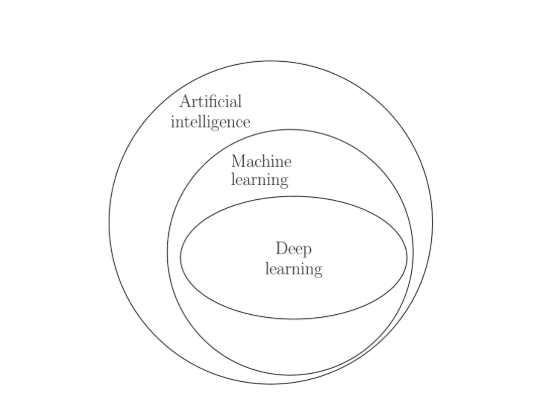
\includegraphics[width=0.7\linewidth]{images/RelatieAI_ML_DL}
    \caption{Relatie tussen AI, ML, en DL  (\cite{Kelleher2019})}
    \label{fig:relatieaimldl}
\end{figure}

\subsection{Machine learning}

Machine learning kan verder onderverdeeld worden in verschillende categorieën, zoals supervised learning, unsupervised learning en reinforcement learning.

\subsection*{Unsupervised learning}

Bij unsupervised learning krijgt het systeem alleen ongelabelde data. Het doel zoals vernoemd werd in \textcite{Naeem2023} is dat het systeem zelf patronen, structuren of groepen in de data ontdekt zonder dat er vooraf een specifieke taak of label is gedefinieerd. Een voorbeeld hiervan is het automatisch groeperen van foto’s van katten zonder dat de foto’s als zodanig zijn gemarkeerd.

\subsection*{Reinforcement learning}

In reinforcement learning leert een systeem door interacties met zijn omgeving, waarbij het probeert acties te ondernemen die de hoogste beloning oplevert. Dit proces wordt gestuurd door de "reward function", die bepaalt wat als goed of slecht wordt beschouwd voor het systeem. De reward function is vast en kan niet worden aangepast door het systeem zelf. Zoals in \textcite{Gallistel1999} vernoemd werd, helpt deze functie het systeem te sturen in het vinden van de beste strategie om zijn prestaties te verbeteren.


\vspace{20 mm}

\subsection*{Supervised learning}

Supervised Learning is een techniek binnen machine learning waarbij een model wordt getraind met gelabelde data. Het leert patronen te herkennen in de gegevens om vervolgens voorspellingen te doen voor nieuwe, onbekende data. Volgens \textcite{Fabris2017} maakt supervised machine learning gebruik van de kenmerken en annotaties in de trainingsset om een model te ontwikkelen dat de annotaties van de testset kan voorspellen. Deze methode is niet alleen nuttig voor voorspellingen, maar kan ook helpen bij het ontdekken van interpreteerbare kennis. Een voorbeeld hiervan is het classificeren van eiwitten als verouderingsgerelateerd (bron).

\subsection{Regressie modellen}

Regressiemodellen worden gebruikt om de relatie tussen een afhankelijke variabele en één of meer onafhankelijke variabelen te begrijpen. Het doel is om een voorspelling te doen over de afhankelijke variabele op basis van de waarden van de andere variabelen. Regressie wordt vaak gebruikt om trends te analyseren en toekomstige uitkomsten te voorspellen.

\subsection*{Random Forest}
Het Random Forest-model is een krachtig en populair machine learning-model dat wordt gebruikt voor zowel classificatie als regressie. Het algoritme maakt gebruik van een verzameling besluitbomen (decision trees) die willekeurig worden gegenereerd — vandaar de naam Random Forest. Elke boom in het model wordt opgebouwd op basis van een willekeurige selectie van features bij elk knooppunt. Deze willekeurigheid zorgt voor variatie tussen de bomen, waardoor het risico op overfitting afneemt en de nauwkeurigheid van het model toeneemt. Volgens \textcite{Sekhar2016} kan je het random forrest proces in de volgende stappen opsplitsen:



\subsection*{Support Vector Machine}

Volgens \textcite{RodriguezPerez2022} zijn Support Vector Machine (SVM) is een krachtig machine learning algoritme dat oorspronkelijk werd ontwikkeld door Vapnik in 1979. Het algoritme werd eerst ontworpen voor binaire classificatieproblemen, waarbij het doel is om objecten in twee categorieën te verdelen. Later werd het uitgebreid naar regressieproblemen, wat bekend staat als Support Vector Regression (SVR).

\vspace{1em}

Wat SVM onderscheidt van andere algoritmes is de manier waarop het werkt met data. Het algoritme projecteert de trainingsdata in een vooraf gedefinieerde feature space, waarin het op zoek gaat naar een hypervlak dat de verschillende klassen optimaal van elkaar scheidt. Als zo’n scheiding in de oorspronkelijke ruimte niet mogelijk is, dan wordt de data getransformeerd naar een ruimte met hogere dimensies waar een lineaire scheiding wél haalbaar kan zijn.

\vspace{1em}

Een belangrijk aspect van SVM is het gebruik van de zogenaamde soft margin variant. Deze laat toe dat sommige punten aan de verkeerde kant van het hypervlak liggen om zo een beter generaliserend model te bekomen. Dit maakt SVM robuuster voor data die niet perfect lineair scheidbaar zijn.

\subsection*{Lineaire regressie}

Lineaire regressie is een veelgebruikte en eenvoudige methode om verbanden tussen meerdere variabelen te analyseren en voorspellingen te doen. Het model wordt vaak toegepast vanwege de duidelijkheid en controle die het biedt in vergelijking met complexere machine learning-modellen.\autocite{Etemadi2021}
\vspace{1em}

Lineaire regressie onderzoekt hoe veranderingen in een afhankelijke variabele verklaard kunnen worden door meerdere onafhankelijke variabelen. Dit kan voor twee doelen worden ingezet:


Deze methode wordt breed toegepast in domeinen zoals geneeskunde, techniek, energie, financiën en milieuwetenschappen. Zo werd lineaire regressie bijvoorbeeld gebruikt om COVID-19 trends te voorspellen, luchtvervuiling te koppelen aan ziekenhuisopnames, en energieverbruik in gebouwen te schatten.

\vspace{1em}

Dankzij zijn eenvoud en flexibiliteit blijft lineaire regressie een krachtig hulpmiddel voor zowel verklarende als voorspellende analyses.


\subsection*{XGBoost}

XGBoost is een krachtig en efficiënt algoritme voor machine learning dat gebaseerd is op het principe van gradient boosting. Het is ontworpen om snel en schaalbaar te zijn, waardoor het goed presteert op grote en complexe datasets. Het model werkt door meerdere eenvoudige beslissingsbomen te combineren. Elke nieuwe boom probeert de fouten van de vorige te verbeteren, waardoor het model stapsgewijs steeds nauwkeuriger wordt. Dankzij optimalisaties zoals parallelle verwerking en slimme technieken om het leerproces te versnellen, is XGBoost een populaire keuze.\autocite{Hakkal2024}

\subsection{Forecast modellen}

Forecast modellen zijn technieken die worden gebruikt om toekomstige waarden te voorspellen op basis van historische gegevens. Ze houden rekening met patronen zoals trends en seizoensgebonden fluctuaties voor nauwkeurige voorspellingen te doen.

\subsection*{SARIMA}

SARIMA is een voorspellingsmodel dat wordt gebruikt om tijdsreeksen te analyseren en toekomstige waarden te schatten. Het is een uitbreiding van het ARIMA-model, dat kijkt naar patronen in de vroegere waarden van een reeks. ARIMA werkt goed voor data zonder duidelijke seizoensinvloeden, maar wanneer er wél sprake is van terugkerende patronen, zoals elke maand of elk kwartaal, is SARIMA beter geschikt \autocite{KumarDubey2021}.

\vspace{1em}

SARIMA bestaat uit twee delen: een niet-seizoensgebonden deel (ARIMA) en een seizoensgebonden uitbreiding. Het model gebruikt verschillende parameters om de juiste voorspelling te maken. Zo geeft het aan hoeveel eerdere waarden (lags) gebruikt worden, hoeveel keer het verschil moet worden genomen om de data stabiel te maken, en hoeveel fouten uit het verleden worden meegenomen.

\vspace{1em}

Het maken van een SARIMA-model gebeurt in een aantal stappen. Eerst wordt gecontroleerd of de data stabiel is (stationair), wat betekent dat het gemiddelde en de spreiding niet veranderen over tijd. Als dat niet zo is, wordt de reeks aangepast door er verschillen van te nemen, net zo lang tot deze stabiel is. Daarna worden er modellen opgebouwd met behulp van patronen in de data. Pas als dat klaar is, kan de voorspelling gemaakt worden. Tot slot wordt gecontroleerd of de voorspelling klopt door de uitkomsten te vergelijken met echte waarden.

\vspace{1em}

SARIMA is handig voor situaties waarin je wilt voorspellen op basis van herhalende patronen in de tijd, zoals verkoop per maand of temperatuur per seizoen \autocite{KumarDubey2021}.

\subsection{Segmentatie modellen}

Segmentatiemodellen worden gebruikt om een groep op te delen in kleinere, vergelijkbare groepen. Dit helpt om patronen te vinden en gerichte acties te ondernemen voor verschillende groepen.

\subsection*{K-means}

Volgens \textcite{Hu2023} is K-means een populaire techniek voor het clusteren van gegevens, waarbij een verzameling van n observaties wordt verdeeld in k groepen. Elk gegevenspunt wordt toegewezen aan de groep waarvan het centrum het dichtstbij ligt. Dit proces gaat door totdat de posities van de centroïden stabiel blijven en de variatie binnen de clusters geminimaliseerd is. Het algoritme werkt iteratief: in de eerste stap worden de punten aan een willekeurig gekozen centrum toegewezen. Vervolgens worden de centra aangepast op basis van de nieuwe groepering, en dit proces wordt herhaald totdat de indeling niet meer verandert.

\subsection*{K-modes}

Het K-modes algoritme volgens \textcite{Kuo2021} is een clustering-algoritme dat specifiek is ontwikkeld voor categorische data. Het is een aanpassing van het K-means algoritme. De belangrijkste verschillen tussen K-means en K-modes zijn:



K-modes is ideaal voor datasets met alleen categorische gegevens, omdat het beter past bij de eigenschappen van deze variabelen en helpt bij het ontdekken van patronen die moeilijk te clusteren zouden zijn met traditionele methoden.

\subsection*{DBScan}

DBSCAN is volgens \textcite{Hanafi2022} een bekend en veelgebruikt algoritme dat groepen maakt op basis van hoe dicht punten bij elkaar liggen. In vergelijking met andere methodes om data te groeperen, heeft DBSCAN enkele sterke punten. Zo kan het groepen herkennen die niet netjes rond of vierkant zijn, het kan losse of afwijkende punten makkelijk opsporen, en het bepaalt automatisch hoeveel groepen er zijn zonder dat je dat vooraf hoeft aan te geven.

\vspace{1em}

Toch heeft DBSCAN ook nadelen. Een belangrijk probleem is dat het traag werkt bij grote hoeveelheden data. Hoe meer gegevens er zijn, hoe langer het duurt om voor elk punt te bepalen welke andere punten in de buurt liggen en hoe dicht die bij elkaar zitten. Hierdoor is het belangrijk om manieren te zoeken om DBSCAN sneller te laten werken, zodat het ook geschikt blijft voor grote datasets.

\vspace{1em}

Het algoritme werkt als volgt: DBSCAN begint met een willekeurig punt uit de dataset dat nog niet eerder is bekeken. Daarna wordt gekeken hoeveel andere punten er binnen een bepaalde afstand (ε) van dit punt liggen. Als er te weinig punten dichtbij liggen (minder dan een minimum aantal, MinPts), wordt het punt gezien als ruis. Ligt het aantal wel boven die grens, dan wordt het punt een kernpunt en begint het algoritme een nieuwe cluster.

Alle punten die in de buurt liggen van dit kernpunt worden verzameld in een lijst. Voor elk van deze punten wordt opnieuw gekeken of het ook een kernpunt is. Als dat zo is, worden zijn buren ook toegevoegd aan de lijst, zodat de cluster zich verder uitbreidt. Als een punt geen kernpunt is, krijgt het alleen het label van de cluster maar wordt er niet verder gezocht vanuit dat punt. Dit proces gaat door tot de lijst leeg is. Daarna kiest het algoritme opnieuw een willekeurig punt dat nog niet is bekeken en herhaalt het proces, tot alle punten in de dataset zijn behandeld.\autocite{Hanafi2022}

\subsection{Deep learning}

Deep learning is een subcategorie binnen Artificial Intelligence die zich richt op het ontwikkelen van grote neurale netwerken die in staat zijn om nauwkeurige beslissingen te nemen. Deep learning is best geschikt voor situaties waar de data complex is en grote datasets beschikbaar zijn. Vandaag de dag maken de meeste online bedrijven gebruik van deep learning. Voorbeelden hiervan zijn Facebook, dat deep learning gebruikt om tekst in online gesprekken te analyseren, en Google, dat deep learning inzet voor afbeeldingszoekopdrachten. Moderne smartphones bevatten deep learning-systemen voor toepassingen zoals gezichtsherkenning en spraakherkenning. \autocite{Kelleher2019}

%\begin{figure}
%  \centering
%  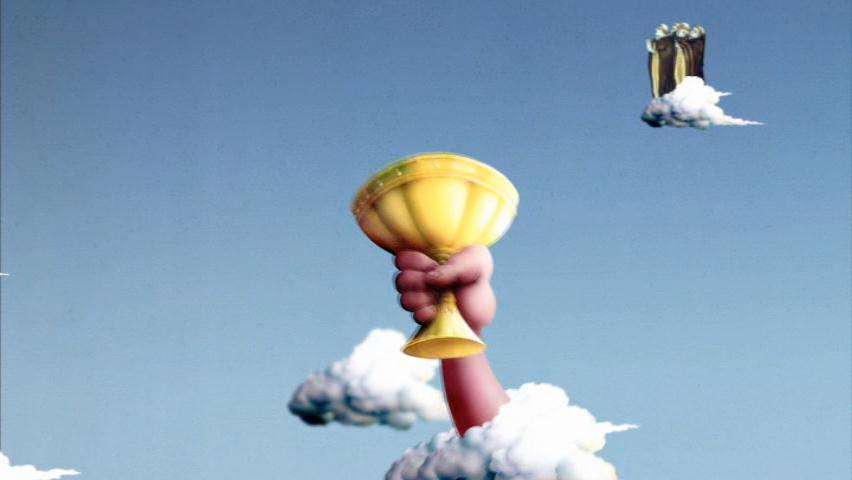
\includegraphics[width=0.8\textwidth]{grail.jpg}
%  \caption[Voorbeeld figuur.]{\label{fig:grail}Voorbeeld van invoegen van een figuur. Zorg altijd voor een uitgebreid bijschrift dat de figuur volledig beschrijft zonder in de tekst te moeten gaan zoeken. Vergeet ook je bronvermelding niet!}
%\end{figure}



%\begin{listing}
%%  \begin{minted}{python}
%%    import pandas as pd
%%    import seaborn as sns
%
%   % penguins = sns.load_dataset('penguins')
% %   sns.relplot(data=penguins, x="flipper_length_mm", y="bill_length_mm", hue="species")
%  %\end{minted}
%  \caption[Voorbeeld codefragment]{Voorbeeld van het invoegen van een codefragment.}
%\end{listing}






%\begin{table}
%  \centering
%  \begin{tabular}{lcr}
%    \toprule
%    \textbf{Kolom 1} & \textbf{Kolom 2} & \textbf{Kolom 3} \\
%    $\alpha$         & $\beta$          & $\gamma$         \\
%    \midrule
%    A                & 10.230           & a                \\
%    B                & 45.678           & b                \\
%    C                & 99.987           & c                \\
%    \bottomrule
%  \end{tabular}
%  \caption[Voorbeeld tabel]{\label{tab:example}Voorbeeld van een tabel.}
%\end{table}


%%=============================================================================
%% Methodologie
%%=============================================================================

\chapter{\IfLanguageName{dutch}{Methodologie}{Methodology}}%
\label{ch:methodologie}

%% TODO: In dit hoofstuk geef je een korte toelichting over hoe je te werk bent
%% gegaan. Verdeel je onderzoek in grote fasen, en licht in elke fase toe wat
%% de doelstelling was, welke deliverables daar uit gekomen zijn, en welke
%% onderzoeksmethoden je daarbij toegepast hebt. Verantwoord waarom je
%% op deze manier te werk gegaan bent.
%% 
%% Voorbeelden van zulke fasen zijn: literatuurstudie, opstellen van een
%% requirements-analyse, opstellen long-list (bij vergelijkende studie),
%% selectie van geschikte tools (bij vergelijkende studie, "short-list"),
%% opzetten testopstelling/PoC, uitvoeren testen en verzamelen
%% van resultaten, analyse van resultaten, ...
%%
%% !!!!! LET OP !!!!!
%%
%% Het is uitdrukkelijk NIET de bedoeling dat je het grootste deel van de corpus
%% van je bachelorproef in dit hoofstuk verwerkt! Dit hoofdstuk is eerder een
%% kort overzicht van je plan van aanpak.
%%
%% Maak voor elke fase (behalve het literatuuronderzoek) een NIEUW HOOFDSTUK aan
%% en geef het een gepaste titel.



\section{Data verzameling}


In deze fase wordt de benodigde data verzameld voor de klantsegmentatie en de salesvoorspellingen uit te voeren. De gegevens komen uit interne bronnen om een compleet overzicht van het klantgedrag en de verkoop te verkrijgen.

\vspace{1 em}

De focus ligt op het verzamelen van de verkoop- en artikeldata van Isopartner Nederland, een entiteit binnen IPCOM NV, aangezien deze data de meest accurate en betrouwbare bron vormt voor het opzetten van een proof of concept. De verzamelde data omvat transactiebedragen, marges, artikeldata, klant-ID en de datum van de  transactie. Het doel is om alle data dat een inzicht zou geven in het koopgedrag van de klant en voor het voorspellen van toekomstige sales te verzamelen. 

\vspace{1 em}

Daarnaast wordt er interne data verzameld die Isopartner Nederland momenteel niet heeft, namelijk gegevens over het aantal werkbare werkdagen per maand. Dit is van belang omdat het aantal werkdagen in een maand invloed kan hebben op de verkoopresultaten, bijvoorbeeld doordat langere maanden met meer werkdagen doorgaans tot hogere verkopen leiden. Deze gegevens zullen persoonlijk opgevraagd worden bij de contactpersonen binnen het bedrijf.

\vspace{1 em}

Op het einde van deze fase is alle nodige data verzameld en beschikbaar voor gebruik. Aangezien meeste data al beschikbaar is in de dataflows van Microsoft Fabric, wordt er voor deze fase 2 weken verwacht.

\newpage

\section{Data-integratie en voorbereiding}


Nadat alle data verzameld is in fase 1, worden de verschillende gegevensbronnen samengevoegd en voorbereid voor verdere analyses. Het doel is om een consistente dataset te creëren die gebruikt kan worden voor klantsegmentatie en salesvoorspellingen.

\vspace{1 em}

De verkoopdata, artikeldata, klantdata en de data over aantal werkdagen per maand worden samengebracht in één dataflow binnen de Microsoft Fabrics omgeving. Deze data wordt vervolgens opgeslagen en verder geoptimaliseerd in een lakehouse binnen dezelfde Microsoft Fabric-omgeving.

\vspace{1 em}

Na het succesvol wegschrijven van de data, wordt er verder gewerkt aan het identificeren van potentiële foutieve data die niet gebruikt mag worden voor analyses. Dit omvat het opsporen van ontbrekende waarden, dubbele records of onjuiste gegevens. Hiervoor wordt gebruikgemaakt van Machine Learning Notebooks binnen Microsoft Fabric, waarbij Python-libraries zoals Panda’s worden toegepast om foutieve data te detecteren en aan te passen. Waar mogelijk worden deze correcties direct doorgevoerd in de dataflows, zodat de gegevens in een goede staat beschikbaar zijn voor verdere verwerking en analyse.

\vspace{1 em}

Het eindproduct van deze fase zou een consistente dataset zijn, gereed voor verdere analyses en modellering. De geschatte tijdsduur voor deze fase is 1 week en 3 dagen.

\newpage

\section{Salesvoorspellingen met regressiemodellen}


Het doel van deze fase is het ontwikkelen van regressiemodellen voor salesvoorspellingen zonder het gebruik van klantsegmentatie, zodat de prestaties later vergeleken kunnen worden met modellen waarin klantsegmentatie wel is opgenomen.

\vspace{1 em}

Dit wordt bereikt door verschillende regressiemodellen toe te passen, zoals XGBoost, lineaire regressie en Random Forest-regressie, met behulp van Python-libraries. Elk model wordt geëvalueerd op basis van prestatiemaatstaven zoals Mean Squared Error (MSE), Root Mean Squared Error (RMSE) en Mean Absolute Error (MAE). De modellen worden getest met een train-test splitsing en cross-validatie, zodat wordt gegarandeerd dat het gekozen model goed generaliseert naar nieuwe data en overfitting wordt voorkomen.

\vspace{1 em}

Daarnaast wordt tijdens deze fase ook SARIMA als forecastmodel toegepast, om een vergelijking te kunnen maken tussen regressiemodellen en tijdreeksvoorspellingen.

\vspace{1 em}

Het uiteindelijke resultaat van deze fase zijn drie verschillende regressiemodellen, die later zullen dienen als basis voor de fase Regressiemodellen met klantsegmentatie, waarin wordt onderzocht hoe klantsegmentatie de precisie van voorspellingen beïnvloedt. Daarnaast is er ook een tijdreeksmodel ontwikkeld, maar alleen de regressiemodellen worden meegenomen naar de volgende fase. De deelvragen die worden beantwoord in deze fase zijn: "Welke regressiemodellen presteren het best bij het voorspellen van sales?" en "Wat is efficiënter bij het voorspellen van sales, forecastmethoden zoals SARIMA of regressiemodellen?". Deze fase duurt twee weken.

\newpage

\section{Klantsegmentatie}


In deze fase ligt de focus op het toepassen van clusteringtechnieken met als doel het opzetten van een volledig clusteringmodel voor klantsegmentatie. Het doel is om betekenisvolle klantsegmenten te creëren op basis van klantendata.


\vspace{1 em}

In deze fase ligt de focus op het toepassen van clusteringalgoritmes zoals K-Means, Gaussian Mixture Models (GMM), DBSCAN en K-Modes met behulp van Scikit-learn, om klanten op basis van hun data in segmenten te groeperen. De resultaten van deze clusteringalgoritmes worden in de fase Regressiemodel met klantsegmentatie vergeleken op basis van hoe goed de verkregen klantsegmenten de precisie van het regressiemodel verbeteren.

\vspace{1 em}

Het eindresultaat van deze fase is het creëren van drie numerieke clusteringmodellen en één categorisch model op basis van klantinformatie en productinformatie. Deze modellen zullen klantsegmenten identificeren, die de basis vormen voor het verder verfijnen van salesvoorspellingen. Voor deze fase wordt een tijdsduur van 3 weken verwacht.


\newpage

\section{Regressiemodel met klantsegmentatie}


In deze fase worden alle regressiemodellen met alle segmentatiemodellen samengebracht om te onderzoeken of het toevoegen van klantsegmentatie leidt tot verbeterde salesvoorspellingen. Dit wordt bereikt door de clusterinformatie toe te voegen, zodat er voorspellingen per cluster per maand worden gemaakt. Daarna worden alle voorspellingen weer samengevoegd om de precisie van het model te meten aan de hand van de Mean Squared Error (MSE), Root Mean Squared Error (RMSE) en Mean Absolute Error (MAE).


\vspace{1 em}

Het eindresultaat van deze fase bestaat uit 12 regressiemodellen, gecombineerd met segmentatiemodellen, die op basis van de vastgestelde maatstaven met elkaar vergeleken kunnen worden. De hoofdonderzoeksvraag, "Kan klantsegmentatie op basis van aankoopgedrag de nauwkeurigheid van salesvoorspellingen verbeteren?", wordt beantwoord. 

\vspace{1 em}

Daarnaast worden de volgende deelvragen beantwoord: “Welke clusteringtechnieken, zoals K-means, GMM, DBSCAN en K-Modes, leveren de meest betekenisvolle klantsegmenten op voor het verbeteren van salesvoorspellingen?”, “Welke regressiemodellen presteren het best bij het voorspellen van sales in combinatie met klantsegmentatie?” en “Hoe kan klantsegmentatie effectief worden geïntegreerd in een regressiemodel voor salesvoorspellingen om de nauwkeurigheid te verbeteren?” Deze fase duurt 2 weken.

%%=============================================================================
%% Methodologie
%%=============================================================================

\chapter{\IfLanguageName{dutch}{Proof of concept}{Proof of concept}}%
\label{ch:Proof of concept}


\section{Introductie}

In dit hoofdstuk wordt een proof of concept ontwikkeld om de onderzoeksvraag van deze bachelorproef te bewijzen. De uitvoering heeft plaatsgevonden binnen de Microsoft Fabric-omgeving, waarbij gebruik werd gemaakt van notebooks, Dataflows Gen2 en Lakehouses. In de proof of concept worden meerdere voorspellingsmodellen opgebouwd en vergeleken om eerst het model met de hoogste precisie te bepalen, zonder segmentatie. Vervolgens worden al deze modellen gecombineerd met verschillende segmentatiemodellen om te onderzoeken hoe klantsegmentatie de nauwkeurigheid van elk regressiemodel beïnvloedt, en of segmentatie daadwerkelijk bijdraagt aan een hogere precisie.

\newpage	

\section{Data verzameling}


Tijdens deze fase van de ontwikkeling van de proof of concept is het essentieel om de vereiste gegevens te verzamelen. Voor het voorspellingsmodel zijn diverse gegevens van groot belang. 

\vspace{1 em}

Allereerst is de SalesInvoice Data van Isopartner Nederland essentieel, omdat deze de verkooptransacties duidelijk maakt. Daarnaast wordt artikeldata en klantdata van Isopartner Nederland gebruikt om een beter beeld te krijgen van de producten en klanten. Tot slot zijn de werkdagen per maand van Isopartner Nederland van belang, om aan te tonen op hoeveel dagen facturen geboekt kunnen worden.

\vspace{1 em}

Voor het verzamelen van de SalesInvoice Data werd contact opgenomen met de bedrijfsleider van Isopartner NL. Er wordt gebruik gemaakt van een live verbinding met het ERP-systeem, waardoor directe toegang tot de meest recente gegevens mogelijk is. Er is een SQL-view geschreven die het verwerken en gebruiken van de data vereenvoudigt. Deze view bevatte aanvullende data die niet direct nodig was voor deze bachelorproef, maar die wel relevant is voor de financiële dataflows die binnen het bedrijf worden gebruikt. Deze data werd eruit gefilterd.

\vspace{1 em}

Voor de klant en artikelgegevens was geen extra view nodig, omdat deze databronnen al beschikbaar waren en rechtstreeks geraadpleegd konden worden.

\vspace{1 em}

De werkdagen per maand zijn gecreëerd op basis van een Excel-bestand waarin de feestdagen staan die Isopartner NL viert. Met deze lijst is handmatig opgezocht wanneer elke feestdag valt en toegevoegd aan een ander Excel-bestand dat alle datums bevat waarop een feestdag valt, van 2020 tot 2026. Deze gegevens worden later in stap 2 gebruikt in een dataflow om voor elke maand het aantal werkdagen erin te berekenen, rekening houdend met de feestdagen en weekenden.

\newpage	

\section{Data-integratie en voorbereiding}

In deze fase zijn de verschillende databronnen met elkaar verbonden en voorbereid voor gebruik in het salesvoorspellingsalgoritme. Dit werd bereikt door het opzetten van Dataflows Gen2 binnen de Microsoft Fabric-omgeving, waarbij de verzamelde data, zoals de SalesInvoice Data, klant- en artikeldata en werkdagendata, werden samengevoegd en geoptimaliseerd voor verdere verwerking. Na het verwerken van de data werden de resultaten opgeslagen in een Lakehouse, een centraal data-opslagsysteem dat zowel gestructureerde als ongestructureerde data ondersteunt. Dit stelde de mogelijkheid in om de data te gebruiken in de notebooks van Microsoft Fabric en de volgende fases van de proof of concept uit te voeren.



\vspace{1 em}

De opbouw van de dataflows binnen dit proof of concept kan worden ingedeeld in drie categorieën: Base Dataflows, Background Dataflows en Output Dataflows die uiteindelijk naar het Lakehouse worden geschreven. Deze structuur zorgt voor een duidelijke scheiding tussen ruwe brongegevens, de tussentijdse verwerking van de data en de uiteindelijke gegevens die gebruikt worden in de analyse.


\subsection{Background Dataflows}

De Background Dataflows bevatten ondersteunende data die nodig is om bepaalde bewerkingen of verrijkingen in andere dataflows mogelijk te maken. Deze dataflows worden niet rechtstreeks gebruikt in het eindresultaat, maar zorgen ervoor dat de base of output dataflows de juiste info ter beschikking hebben.

\subsection*{Calender}

Dit is een Background Dataflow die alle extra info bevat die in een DIM Calendar zou zitten. Denk hierbij aan dingen zoals de maand- en weeknummers, jaar, kwartaal, dag van de week, enzovoort.

\subsection*{Article PIM Enrich}

Deze Background Dataflow voegt extra artikelinformatie toe die wel beschikbaar is in het PIM-systeem, maar niet lokaal in het ERP. Denk bijvoorbeeld aan producteigenschappen of classificaties die enkel in PIM worden beheerd. De data uit deze flow wordt later samengevoegd met de artikeldata om zo een meer volledig beeld te krijgen van elk artikel.

\subsection*{Article mappings}

Deze Background Dataflow bevat vier soorten mappings: Original Manufacturer, Competence Center, Product Type en Material Mappings. Het doel hiervan is zorgen dat dingen die eigenlijk hetzelfde bedoelen, maar anders geschreven zijn, toch als éénzelfde waarde worden gezien.

\subsection*{Article master}

Dit is een databron die rechtstreeks connecteert met het ERP-systeem van Isopartner NL. Hier worden verschillende bronnen samengebracht tot één article master. Die wordt later gebruikt in de Article Base Dataflow om alle artikels bij elkaar te hebben.

\subsection*{Customer Mappings}

Deze dataflow bevat 3 mappings: customer conso mappings, customer group mappings en customer country mappings. Zo worden waarden die verschillende namen hebben maar eigenlijk op hetzelfde slaan, netjes omgezet naar één consistente naam.

\subsection*{Transactions}

Deze dataflow bevat de transactiegegevens van 2020 tot 2022, die deel uitmaken van de base dataflow van de sales invoices. Het gaat om alle transactie-informatie die we nodig hebben voor verdere verwerking en analyse in de volgende stappen van de proof of concept.


\subsection{Base Dataflows}

De Base Dataflows vormen het startpunt van het hele dataverwerkingsproces in deze proof of concept. Het gaat hier om de eerste dataflows die de drie belangrijkste databronnen ophalen: de SalesInvoice data, de klantendata en de artikeldata van Isopartner NL. Deze flows halen de ruwe data rechtstreeks uit het bronsysteem en leggen de basis waarop in de volgende stappen verder wordt gebouwd.

\subsection*{Sales Invoices}

Deze dataflow bestaat uit twee hoofdbronnen. De eerste is een historische dataset genaamd Isopartner NL Transactions 2020–2022, die alle salesgegevens uit die periode bevat. De tweede bron is de SQL-view die door Joshua Fransz werd opgesteld. Deze view levert de meest recente salesdata en sluit aan op de structuur van het huidige ERP-systeem. Door beide bronnen te combineren in één dataflow, wordt een volledige en consistente tijdslijn van verkooptransacties opgebouwd die klaar is voor verdere verwerking.

\vspace{1 em}

Om deze dataflow klaar te maken voor het salesvoorspellingsalgoritme, zijn er een aantal bewerkingen uitgevoerd. Eerst zijn de kolomnamen hernoemd zodat alles mooi consistent is over de datasets heen. Daarna zijn kolommen die niet nodig waren eruit gehaald. Ook zijn er nieuwe kolommen toegevoegd, zoals een berekende Margin-kolom. Als laatste is er een filter toegevoegd die rijen weglaat waar zowel de Turnover als de Margin nul zijn, omdat die toch geen waarde hebben voor de analyse.

\subsection*{Customer}

In de Base Dataflow voor klantdata worden vier belangrijke bronnen samengevoegd. De eerste bron is Customer Base, waar de meeste klantinformatie wordt opgeslagen. Vervolgens wordt de Enrich Customer Conso Mapping, die verwijst naar een Background Dataflow, gebruikt om klantnamen naar een uniform formaat te mappen. Dit maakt het mogelijk om duplicaten te identificeren en te beheren. Daarnaast komt de Customer Additional bron met extra klantgegevens die de dataset verder verrijken. Tot slot levert de Customer Group bron klantgroepinformatie. Al deze data wordt samengevoegd tot één eindresultaat: een volledige klantgroep die klaar is voor verdere analyse.

\vspace{1 em}

De stappen die in deze dataflow zijn uitgevoerd, bestaan uit het samenvoegen van de verschillende databronnen en het verwijderen van duplicaten, zodat we een schone en consistente klant bron hebben.

\subsection*{Article}


De base dataflow voor artikels is opgebouwd uit een combinatie van hoofd databron van Isopartner NL en meerdere Excel-bestanden die extra informatie toevoegen. De hoofdbron bevat de basisgegevens van de artikels, terwijl de Excel-bestanden gebruikt worden om extra details toe te voegen.

\vspace{1 em}

De belangrijkste stappen in deze dataflow zijn het samenvoegen van alle databronnen en het structureren van de data zodat ze bruikbaar is in de latere fases van de proof of concept.

\newpage

\subsection{Output Dataflows}

De output dataflows dienen als basis voor het trainen van het model en het maken van voorspellingen. Ze verzamelen en verwerken de verschillende datastromen die door de eerdere fases zijn opgebouwd en zorgen ervoor dat de gegevens klaar zijn voor zowel het trainen van het model als het genereren van de voorspellingen.

\subsection*{Sales prediction data}

In deze dataflow worden vier belangrijke bronnen gecombineerd: de Base Dataflows van article, customer, en sales invoices, samen met de workingdays. Deze data wordt samengevoegd en klaargemaakt voor gebruik in het salesvoorspellingsalgoritme, zodat we een nauwkeurige voorspelling kunnen maken van de toekomstige verkopen. Deze data wordt automatisch weggeschreven naar een Lakehouse voor gebruik in de notebooks.

\subsection*{Prediction Data}

Deze dataflow begint dynamisch vanaf morgen en genereert automatisch toekomstige datums die gelinkt worden met de bijbehorende werkdagen van die maand. Deze data kan vervolgens worden gebruikt voor voorspellingen door het salesvoorspellingsalgoritme. Deze data wordt automatisch weggeschreven naar een Lakehouse voor gebruik in de notebooks.

\newpage

\section{Salesvoorspellings modellen}


In deze fase wordt een salesvoorspellingsalgoritme ontwikkeld, waarbij zowel regressiemodellen als een klassiek forecastmodel met elkaar worden vergeleken. De regressiemodellen die worden gebruikt, zijn Random Forest Regressor, Lineaire Regressie en XGBoost. Daarnaast wordt ook het SARIMA-model (Seasonal AutoRegressive Integrated Moving Average) opgenomen om te onderzoeken hoe een traditioneel tijdreeksmodel presteert ten opzichte van de regressiebenadering. De modellen worden geëvalueerd op basis van foutmaten zoals RMSE (Root Mean Squared Error), MSE (Mean Squared Error) en MAE (Mean Absolute Error). De regressiemodellen, met uitzondering van het SARIMA-model, zullen verder worden geanalyseerd om te onderzoeken hoe klantsegmentatie de nauwkeurigheid van de voorspellingen beïnvloedt.

\subsection{Imports}

\vspace{1 em}

\subsection*{Algemene imports}

In deze sectie worden de basisbibliotheken geïmporteerd die nodig zijn voor dataverwerking, preprocessing en evaluatie van de modellen.

\vspace{1em} % Optionele ruimte voor scheiding tussen tekst en code

\begin{listing}[H]
    \begin{minted}{python}
        import pandas as pd
        import numpy as np
        from sklearn.model_selection import train_test_split
        from sklearn.preprocessing import StandardScaler
        from sklearn.metrics import mean_squared_error, mean_absolute_error
        from deltalake import DeltaTable
    \end{minted}
    \caption[Algemene imports]{Imports voor dataverwerking, preprocessing, evaluatie en Delta Lake.}
\end{listing}

\newpage

\subsection*{Specifieke imports voor de modellen}

In deze sectie worden de specifieke bibliotheken geïmporteerd die nodig zijn voor het trainen van verschillende modellen, zoals Random Forest, SARIMA, XGBoost en lineaire regressie. Doorgaans wordt slechts één van deze modellen per script gebruikt, waardoor enkel de relevante import nodig is voor dat specifieke model.

\vspace{1 em}

Daarnaast is GridSearch toegevoegd voor de Random Forest- en XGBoost-modellen om een geoptimaliseerde training toe te passen via hyperparameterafstemming.



\vspace{1em} 

\begin{listing}[H]
    \begin{minted}{python}
        from sklearn.ensemble import RandomForestRegressor
        from statsmodels.tsa.statespace.sarimax import SARIMAX
        import xgboost as xgb
        import statsmodels.api as sm
        from sklearn.linear_model import LinearRegression
        from sklearn.model_selection import GridSearchCV
    \end{minted}
    \caption[Specifieke imports voor modellen]{Imports voor Random Forest, SARIMA, XGBoost, SVM en Lineaire regressie.}
\end{listing}

\newpage

\subsection{Data inladen}

Voor de training van de modellen en de toekomstige voorspellingen, wordt de benodigde data opgehaald uit het Lakehouse. De "Sales Prediction data" wordt ingeladen en omgezet naar een pandas DataFrame voor het trainen van de modellen. Deze data bevat historische verkoopcijfers die gebruikt worden voor het genereren van de voorspellingen. Dit proces is opgezet in de vorige fases met behulp van de Gen2 dataflows.



\subsection*{Data voorbereiden en preprocessing}

In deze fase wordt de data voorbereid om gebruikt te kunnen worden in de voorspellingsmodellen. De oorspronkelijke dataset, die werd ingeladen vanuit het Lakehouse, bevat verkoopgegevens op transactieniveau. Omdat het doel van dit proof of concept is om voorspellingen te doen op maandbasis, worden de gegevens gegroepeerd per maand. Hiervoor wordt eerst gezorgd dat de datumkolom correct is geformatteerd als een datetime-object. Vervolgens worden nieuwe kolommen aangemaakt op basis van deze datums, zoals maand, jaar en kwartaal.

\vspace{1em} 

De gegroepeerde data wordt schoon gemaakt, waarbij enkel de relevante kolommen blijven. Er wordt ook een filter toegepast om enkel historische data te behouden tot en met de laatste maand waarvoor volledige data beschikbaar is, zodat voorspellingen worden gemaakt op basis van complete gegevens.

\vspace{1em} 

Daarnaast wordt een splitsing gemaakt tussen de trainings- en testgegevens, waarbij 80 procent van de data gebruikt wordt om het model te trainen en 20 procent om het model te evalueren. Om te zorgen dat de verschillende numerieke variabelen vergelijkbaar zijn qua schaal, worden deze gestandaardiseerd met behulp van een StandardScaler. Deze preprocessingstappen zijn essentieel voor de betrouwbaarheid van de machine learning-modellen die in de fase hierna wordt toegepast.

\vspace{1em} 

Voor het SARIMA-model, dat specifiek geschikt is voor tijdreeksvoorspellingen, wordt de datumkolom ingesteld als index van de dataset. Dit is noodzakelijk omdat SARIMA gebruikmaakt van de tijdsstructuur in de data om seizoenspatronen en trends te modelleren. De data wordt daarbij gesorteerd op datum om de chronologische volgorde te behouden.

\subsection{Model training}


In deze fase worden de verschillende modellen getraind en gebruikt om voorspellingen te doen, waaronder lineaire regressie, SVM, XGBoost en Random Forest. Voor zowel het Random Forest- als het XGBoost-model wordt GridSearch toegepast om de optimale hyperparameters te vinden.

\subsection*{Parameter grids en optimale parameters}

\begin{listing}[H]
    \small  % Dit maakt de tekst kleiner
    \begin{minted}{python}
        # Parametergrid voor Random Forest
        param_grid_rf = {
            'n_estimators': [50, 100],             # Aantal bomen in het bos
            'max_depth': [5, 10, None],            # Maximale diepte van de boom
            'min_samples_split': [2, 10],          # Minimaal aantal samples om een interne node te splitsen
            'min_samples_leaf': [1, 5]             # Minimaal aantal samples per blad
        }
        
        # Optimale model (beste hyperparameters) voor Random Forest
        optimal_rf_params = {
            'max_depth': 10,                       # Maximale diepte van de boom
            'min_samples_leaf': 1,                 # Minimaal aantal samples per blad
            'min_samples_split': 2,                # Minimaal aantal samples om een interne node te splitsen
            'n_estimators': 50                    # Aantal bomen in het bos
        }
        
        # Parametergrid voor XGBoost
        param_grid_xgb = {
            'n_estimators': [50, 100],             # Aantal boosting rondes
            'max_depth': [5, 10, None],            # Maximale diepte van de individuele bomen
            'learning_rate': [0.01, 0.1, 0.2],     # Leerpercentage (hoe snel het model leert)
            'subsample': [0.8, 1.0],               # Fractie van de training data die per boom wordt gebruikt
            'colsample_bytree': [0.8, 1.0]         # Fractie van kolommen die per boom worden gebruikt
        }
        
        # Optimale model (beste hyperparameters) voor XGBoost
        optimal_xgb_params = {
            'colsample_bytree': 0.8,               # Fractie van kolommen die per boom worden gebruikt
            'learning_rate': 0.2,                  # Leerpercentage (hoe snel het model leert)
            'max_depth': 10,                       # Maximale diepte van de individuele bomen
            'n_estimators': 50,                    # Aantal boosting rondes
            'subsample': 0.8                       # Fractie van de training data die per boom wordt gebruikt
        }
    \end{minted}
    \caption{Parametergrids voor Random Forest en XGBoost met de optimale hyperparameters}
    \label{lst:parametergrids_optimal}
\end{listing}


\subsection{Model evalueren}

In deze fase worden de prestaties van elk getraind model beoordeeld met behulp van verschillende foutmaten, zoals Mean Squared Error (MSE), Root Mean Squared Error (RMSE) en Mean Absolute Error (MAE). Deze evaluatie geeft inzicht in de nauwkeurigheid van de voorspellingen en maakt het mogelijk om modellen met elkaar te vergelijken. 
 
\vspace{1em} 
 
Daarnaast wordt het laatste jaar gevisualiseerd in een grafiek waarin de voorspelde omzet wordt vergeleken met de werkelijke omzet. Deze visualisatie helpt bij het beoordelen van de kwaliteit van de voorspellingen over tijd.

\subsection*{Prestaties van de Modellen}

\begin{table}[H]
    \centering
    \begin{tabular}{|c|c|c|c|}
        \hline
        \textbf{Model}      & \textbf{MSE}       & \textbf{RMSE}       & \textbf{MAE}       \\ \hline
        Linear              & 202,982,205,716    & 450,535             & 346,951            \\ \hline
        Random Forest       & 242,022,929,294    & 491,598             & 378,430            \\ \hline
        XGBoost             & 282,605,525,485    & 531,607             & 376,649            \\ \hline
        SARIMA              & 751,000,964,364    & 866,603             & 619,703       \\ \hline
    \end{tabular}
    \caption{Evaluatie van de regressiemodellen met MSE, RMSE en MAE}
    \label{tab:model_evaluation}
\end{table}


\subsection*{Grafieken}


\begin{figure}[H]
    \centering
    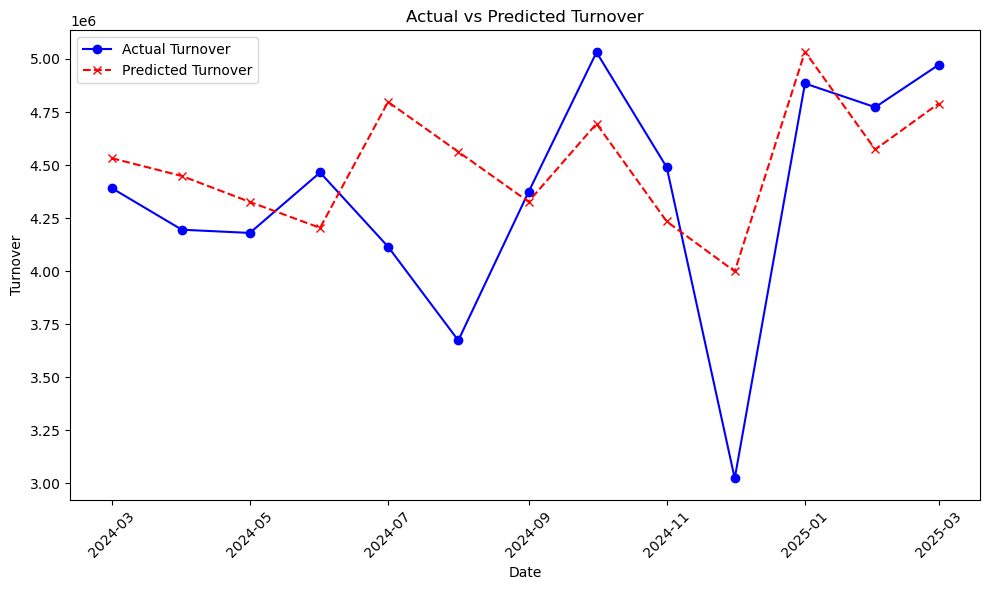
\includegraphics[width=1\linewidth]{images/Linear_Grafiek}
    \caption{Grafiek van het lineaire regressie model}
    \label{fig:GrafiekLinear}
\end{figure}

\begin{figure}[H]
    \centering
    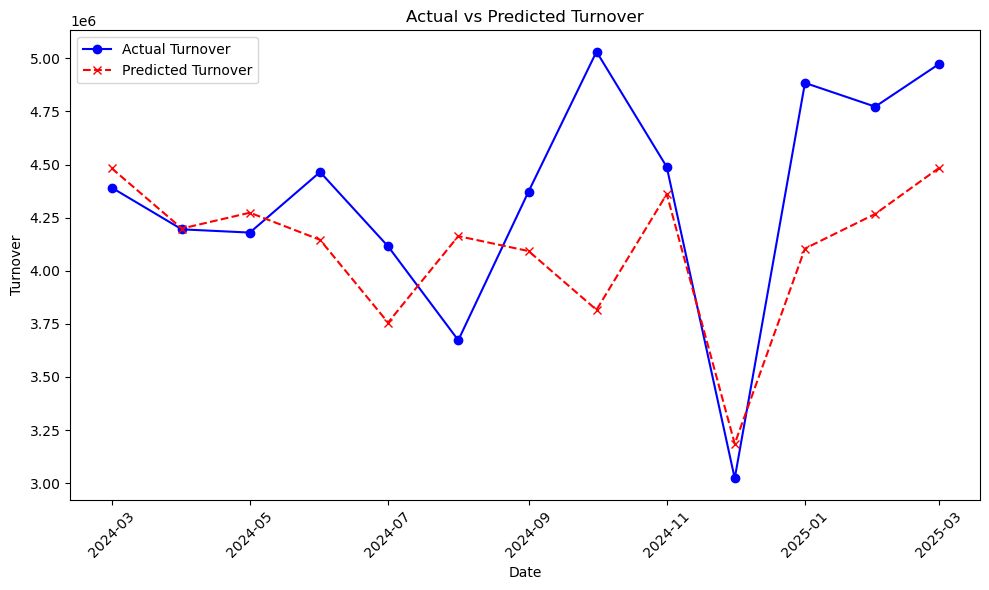
\includegraphics[width=1\linewidth]{images/RandomForrest_Grafiek}
    \caption{Grafiek van het Random Forrest model}
    \label{fig:GrafiekForrest}
\end{figure}

\begin{figure}[H]
    \centering
    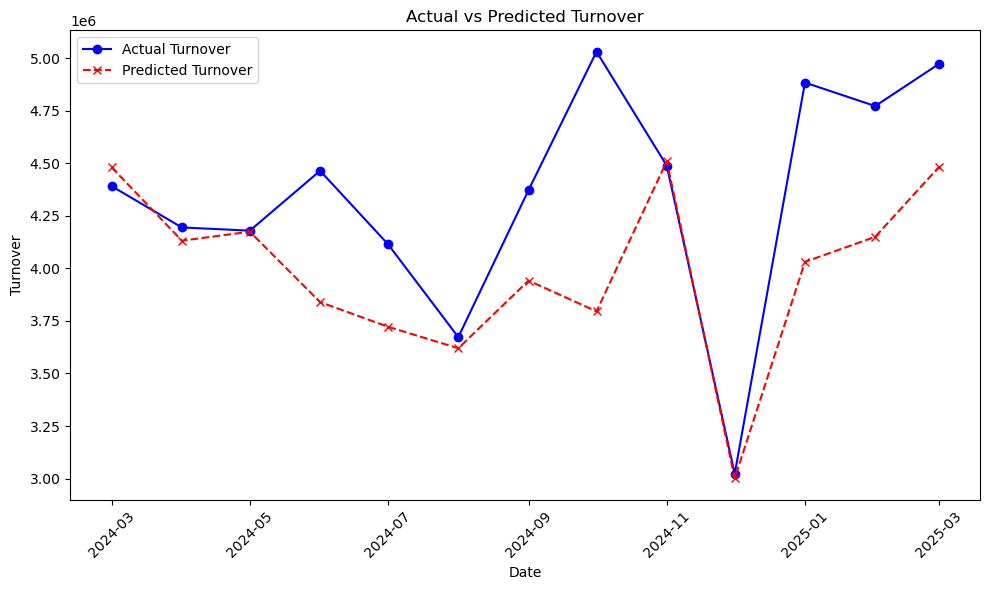
\includegraphics[width=1\linewidth]{images/XGBoost_Grafiek}
    \caption{Grafiek van het XGBoost model}
    \label{fig:GrafiekXGBoost}
\end{figure}

\begin{figure}[H]
    \centering
    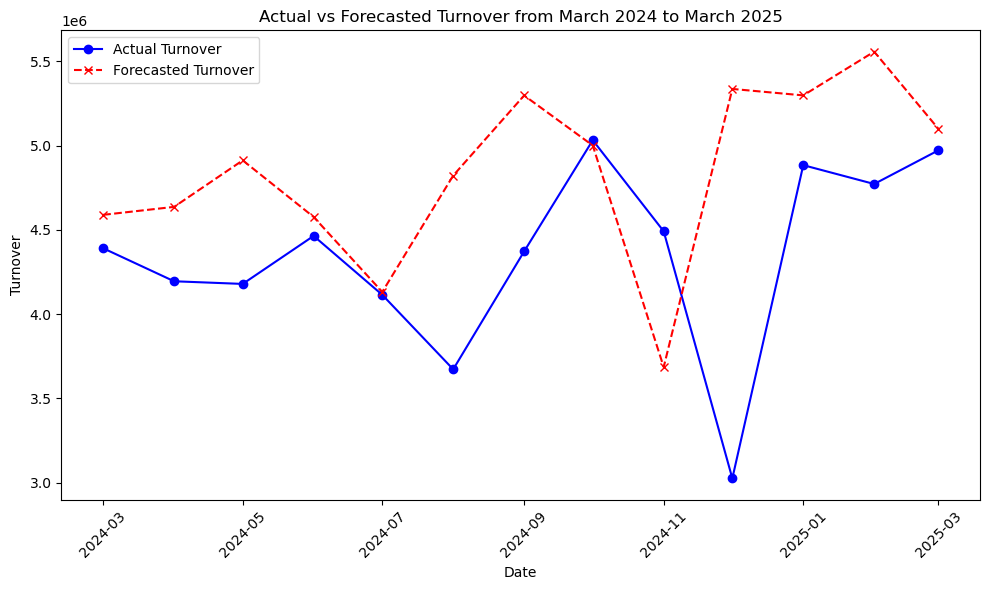
\includegraphics[width=1\linewidth]{images/Samira/Samiragrafiek}
    \caption{Grafiek van het SAMIRA model}
    \label{fig:GrafiekSAMIRA}
\end{figure}

\subsection{Conclusie}

Op basis van de evaluatie van de verschillende modellen blijkt dat lineaire regressie de beste prestaties levert op alle foutmaten (MSE, RMSE en MAE). Hoewel complexere modellen zoals Random Forest en XGBoost vaak betere resultaten kunnen opleveren bij niet-lineaire patronen, bleek lineaire regressie in dit geval het meest geschikt voor deze dataset.

\vspace{1em} 

Daarnaast presteert het SARIMA-model duidelijk slechter dan de andere modellen. Hoewel tijdreeksmodellen zoals SARIMA vaak geschikt zijn voor het modelleren van seizoensgebonden trends en patronen, bleek het in deze situatie minder accuraat bij het voorspellen van de maandelijkse verkoopcijfers.


\newpage

\section{Klantsegmentatie model}

In deze fase van de POC worden verschillende segmentatiemodellen toegepast om klanten te groeperen op basis van hun aankoopgedrag en kenmerken. Er wordt gewerkt met modellen zoals K-Means, DBSCAN, Gaussian Mixture Models (GMM) en K-Modes, die ook categorische klant- en artikeldata meenemen. De clusterdata wordt opgeslagen voor later gebruik in de volgende fase, waarin deze geïntegreerd zal worden met het best presterende salesvoorspellingsalgoritme zonder segmentatie, om te bepalen welk segmentatiemodel de salesvoorspellingen het beste verbetert.

\subsection{Data}

Voor de segmentatiemodellen K-Means, DBSCAN en GMM worden numerieke gegevens gebruikt, zoals totaal gespendeerd bedrag en gemiddeld factuurbedrag. Deze gegevens zijn geschikt voor het identificeren van clusters op basis van het aankoopgedrag van klanten.

\vspace{1em} 

Voor het K-Modes model worden categorische gegevens gebruikt, zoals Customer group, Activity, Competence center en Product type, die inzicht bieden in klantsegmenten op basis van niet-numerieke kenmerken.

\subsection*{Inzicht in de Data}

Deze grafiek toont het totaal gespendeerd bedrag per klant. Het biedt een eerste kijk op het koopgedrag van klanten en helpt om een beter begrip te krijgen van de variatie in uitgaven voordat we de segmentatiemodellen toepassen.

\begin{figure}[H]
    \centering
    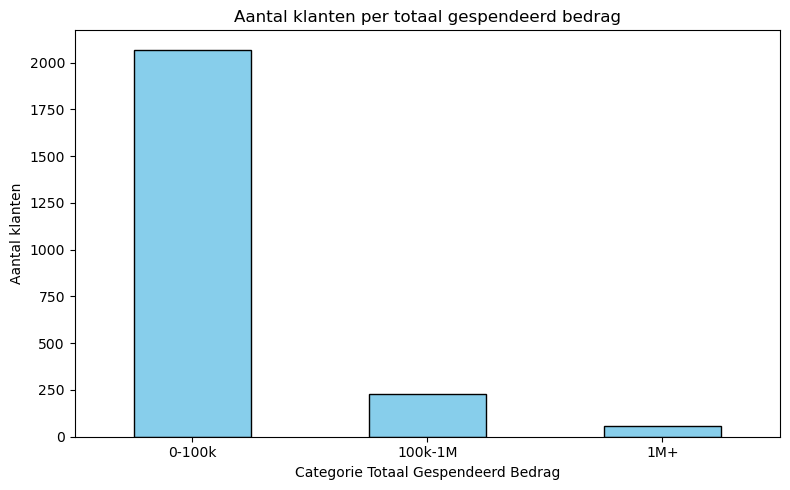
\includegraphics[width=0.8\linewidth]{images/Kmeans/KlantenAnalyse}
    \caption{Klanten per aankoopgroep}
    \label{fig:KlantenPerGroep}
\end{figure}



\subsection{Imports}

\subsection*{Imports voor numerieke segmentatiemodellen}

In deze sectie worden de specifieke bibliotheken geïmporteerd die nodig zijn voor het trainen en evalueren van de numerieke segmentatiemodellen, zoals K-Means, DBSCAN, en Gaussian Mixture Models (GMM). Deze modellen werken met numerieke data.

\vspace{1em}

\begin{listing}[H]
    \begin{minted}{python}
        #Algemene Imports
        import pandas as pd
        import matplotlib.pyplot as plt
        import seaborn as sns
        from sklearn.preprocessing import StandardScaler
        from sklearn.decomposition import PCA
        from deltalake import DeltaTable, write_deltalake
        
        #Specifieke imports per model
        from sklearn.mixture import GaussianMixture
        from sklearn.cluster import KMeans
        from sklearn.cluster import DBSCAN
    \end{minted}
    \caption[Imports voor numerieke segmentatiemodellen]{Imports voor K-Means, DBSCAN en Gaussian Mixture Models.}
\end{listing}

\subsection*{Imports voor categorische segmentatiemodel}

In deze sectie worden de specifieke bibliotheken geïmporteerd die nodig zijn voor het trainen van het K-Modes model, dat geschikt is voor categorische gegevens. Dit model wordt gebruikt om klantgroepen te segmenteren op basis van niet-numerieke kenmerken zoals klantgroep, activiteit en producttype.

\vspace{1em}

\begin{listing}[H]
    \begin{minted}{python}
        import pandas as pd
        import matplotlib.pyplot as plt
        import pyarrow as pa
        from kmodes.kmodes import KModes
        from deltalake import DeltaTable, write_deltalake
    \end{minted}
    \caption[Imports voor K-Modes segmentatiemodel]{Imports voor het K-Modes model.}
\end{listing}


\newpage

\subsection{Segmentatiemodellen}

In de volgende secties wordt uitgelegd hoe de klantgroepen zijn gemaakt en wat de uitkomsten daarvan zijn. Per model wordt beschreven hoe de groepen tot stand kwamen, welke soorten klanten er in elke groep zitten en wat we daaruit kunnen afleiden over hun koopgedrag.

\subsection*{K-Means}


Voor K-Means moet het aantal groepen waarin de data wordt opgedeeld, zelf worden bepaald. Een veelgebruikte manier om dit aantal te kiezen, is de Elbow-methode. Bij deze methode wordt gekeken naar hoe de totale variatie binnen de groepen (de WCSS, oftewel de inertie) afneemt naarmate het aantal clusters toeneemt. In het begin zal de variatie sterk afnemen, maar op een gegeven moment zal het verschil kleiner worden. Het punt waarop deze afname afvlakt, wordt vaak gekozen als het beste aantal clusters. Dit punt wordt het "knikpunt" genoemd.

\vspace{1em}

In de onderstaande grafiek is te zien hoe de WCSS zich gedraagt bij verschillende aantallen clusters. In dit geval is het optimale aantal clusters 3, omdat daar het knikpunt zichtbaar is, wat lijkt op een "elboog".

\begin{figure}[H]
    \centering
    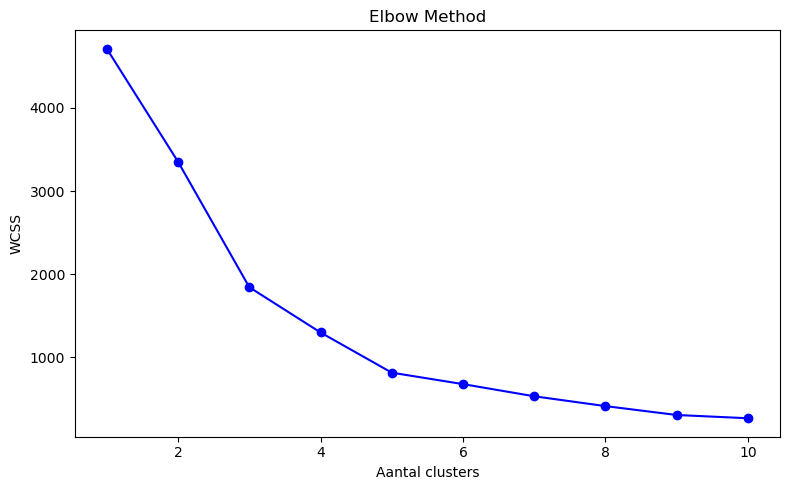
\includegraphics[width=1\linewidth]{images/Kmeans/ElbowMethodKmeans}
    \caption{Elbow method K-means grafiek}
    \label{fig:ElbowMethodKmeans}
\end{figure}


\newpage

\subsection*{K-Modes}

K-Modes is een clusteringtechniek die speciaal ontworpen is voor categorische data. In tegenstelling tot K-Means, dat werkt met numerieke waarden en gebruikmaakt van gemiddelden, bepaalt K-Modes de modus (meest voorkomende waarde) binnen elke groep. Deze methode maakt het mogelijk om categorieën op een logische manier te groeperen zonder dat numerieke afstandsmetingen nodig zijn.

\vspace{1em}

Ook bij K-Modes moet het aantal clusters vooraf worden bepaald. Hiervoor kan een aangepaste versie van de Elbow-methode worden gebruikt, waarbij de kosten (bijvoorbeeld het aantal niet-overeenkomende categorieën binnen clusters) worden geanalyseerd. Het optimale aantal clusters wordt gekozen op het punt waar het toevoegen van extra clusters nauwelijks nog zorgt voor een verdere afname van de kosten.

\vspace{1em}

In de onderstaande grafiek is te zien hoe de kosten zich gedragen bij verschillende aantallen clusters. Het optimale aantal clusters is , omdat hier de afname in kosten aanzienlijk kleiner wordt en verder verhogen van het aantal clusters nauwelijks nog tot een verbetering leidt.


\begin{figure}[H]
    \centering
    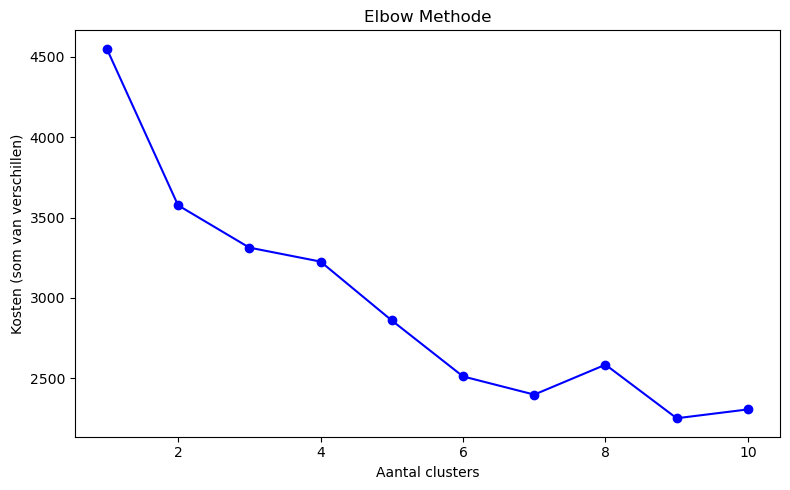
\includegraphics[width=1\linewidth]{images/Kmodes/ElbowmethodKmodes}
    \caption{Elbow method K-modes grafiek}
    \label{fig:ElbowMethodKmodes}
\end{figure}

\newpage

\subsection*{DBSCAN}

Met DBSCAN wordt het aantal clusters automatisch bepaald op basis van de dichtheid van de data. Hierbij worden punten die niet aan de dichtheidscriteria voldoen als outliers (-1) gemarkeerd, terwijl de overige punten in clusters worden ingedeeld. Het aantal clusters wordt dus dynamisch berekend, zonder vooraf gedefinieerde grenzen.

\subsection*{GMM}

Bij GMM wordt het aantal clusters automatisch bepaald door de data te modelleren als een combinatie van meerdere Gaussian distributies. In tegenstelling tot DBSCAN, dat zich richt op dichtheid, gebruikt GMM statistische verdelingen om de optimale clustering van de gegevens te berekenen.

\newpage

\subsection{Resultaten}

Alle clusterdata van elk segmentatiemodel is weggeschreven naar een Lakehouse voor gebruik in fase 5.

\subsection*{Numerieke segmentatiemodellen}

Voor de numerieke segmentatie modellen zijn er drie grafieken gekozen om de prestaties van de clusteringstechnieken te analyseren. Deze grafieken geven inzicht in verschillende aspecten van de clusters en hoe de klanten zijn verdeeld over de verschillende groepen.

\vspace{1em}

De eerste grafiek biedt een visuele weergave van de clusters in een 2D-ruimte. Hierbij worden de eerste twee hoofdcomponenten (bijvoorbeeld PCA1 en PCA2) gebruikt om de klanten te plotten, waarbij elke kleur een cluster vertegenwoordigt.Voor K-Means worden de centroids van de clusters gemarkeerd met een "X", die de centrale punten van de klantgroepen aanduiden. Deze grafiek biedt een overzicht van de verdeling van de klanten over de clusters en toont de centrale punten van elke groep.

\vspace{1em}

De tweede grafiek toont het aantal klanten per cluster. Elke balk in de grafiek representeert het aantal klanten binnen een specifiek cluster. De x-as geeft de clusters weer, terwijl de y-as het aantal klanten binnen elk cluster toont. Deze grafiek maakt het mogelijk om te zien hoe de klanten zijn verdeeld over de clusters en helpt om te begrijpen welke groepen groter of kleiner zijn.

\vspace{1em}

De derde grafiek biedt inzicht in het verband tussen twee variabelen, namelijk het gemiddelde factuurbedrag en het totaal uitgegeven bedrag per klant, opgedeeld per cluster. Op de x-as staat het gemiddelde factuurbedrag per klant, terwijl de y-as het totaal bedrag toont dat een klant heeft uitgegeven. Elke kleur in de grafiek komt overeen met een cluster, waardoor het duidelijk wordt hoe de verschillende klantgroepen zich verhouden op basis van deze twee variabelen.


\subsection*{K-means}

\begin{figure}[H]
    \centering
    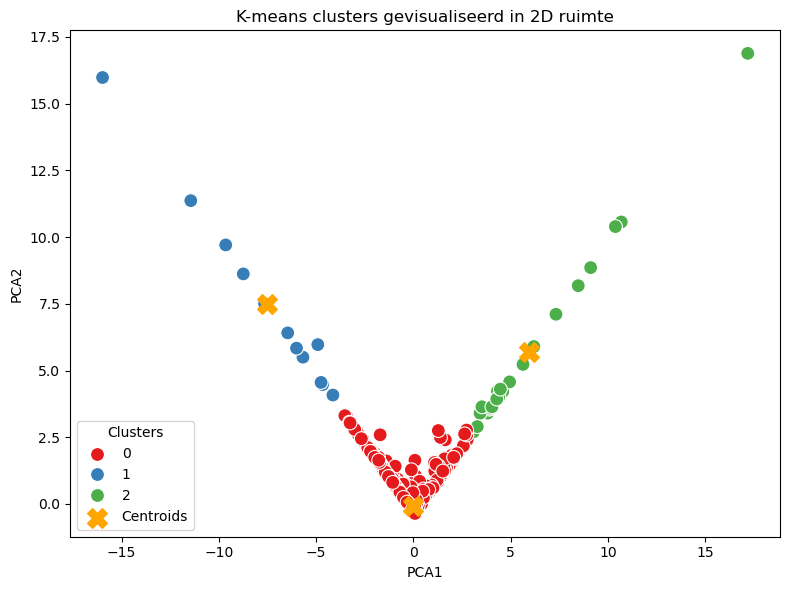
\includegraphics[width=0.8\linewidth]{images/Kmeans/2DrepresentatieKmeans}
    \caption{2D-representatie van de K-Means clusters met PCA en centroids}
    \label{fig:PCA_KMeans}
\end{figure}

\begin{figure}[H]
    \centering
    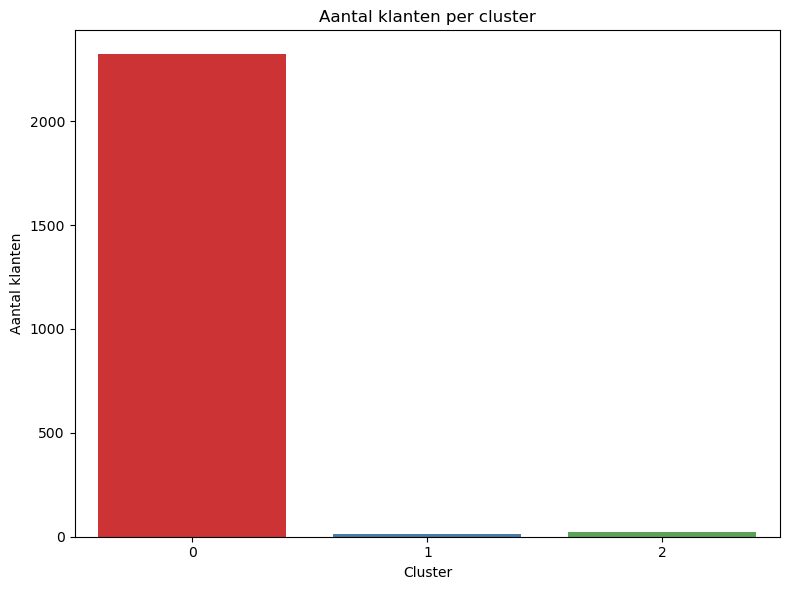
\includegraphics[width=0.8\linewidth]{images/Kmeans/AantalKlantenKMeans}
    \caption{Aantal klanten per cluster (K-Means)}
    \label{fig:Klanten_KMeans}
\end{figure}

\begin{figure}[H]
    \centering
    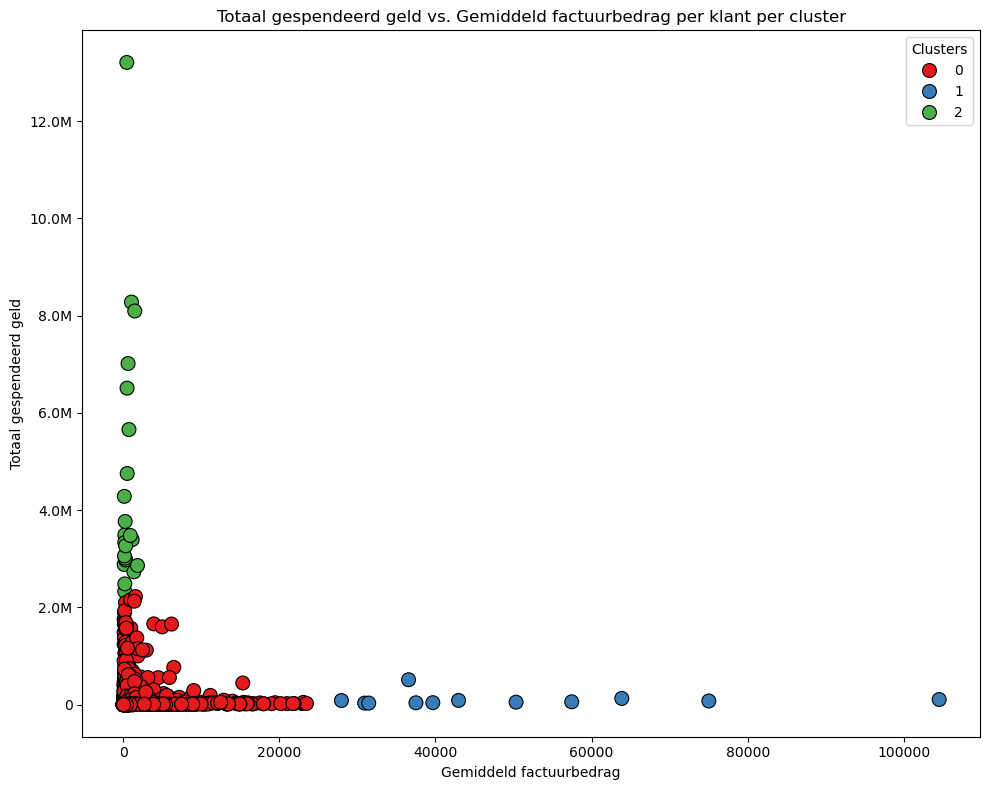
\includegraphics[width=0.8\linewidth]{images/Kmeans/KMeansClusterAnalyse}
    \caption{Analyse van gemiddelde factuurbedrag vs. totaal gespendeerd bedrag per klant (K-Means)}
    \label{fig:Analyse_KMeans}
\end{figure}

\subsection*{GMM}

\begin{figure}[H]
    \centering
    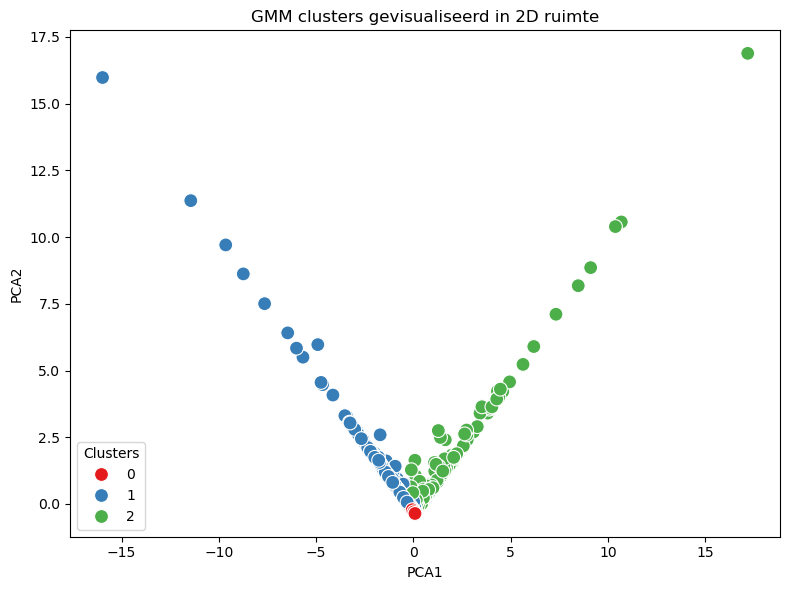
\includegraphics[width=0.8\linewidth]{images/GMM/AnalyseGMM}
    \caption{2D-representatie van de GMM clusters met PCA}
    \label{fig:PCA_GMM}
\end{figure}

\begin{figure}[H]
    \centering
    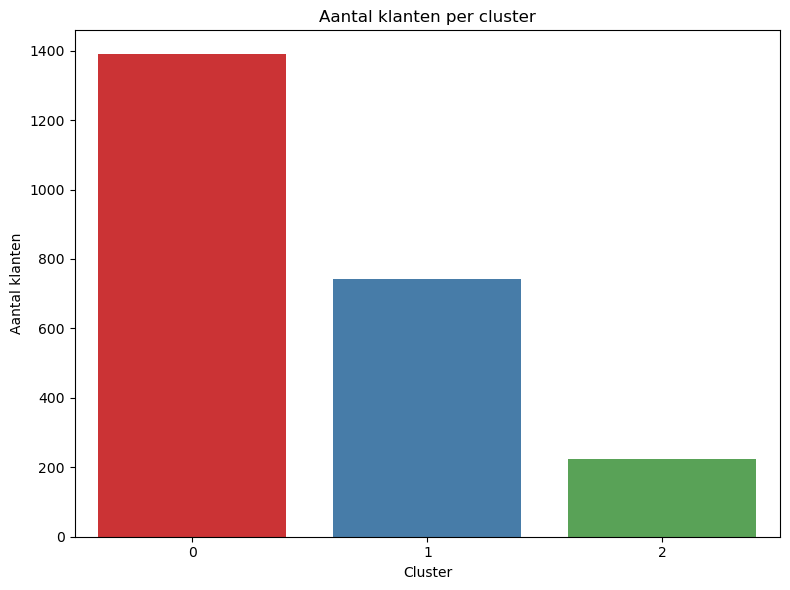
\includegraphics[width=0.8\linewidth]{images/GMM/AantalKlantenGMM}
    \caption{Aantal klanten per cluster (GMM)}
    \label{fig:Klanten_GMM}
\end{figure}

\begin{figure}[H]
    \centering
    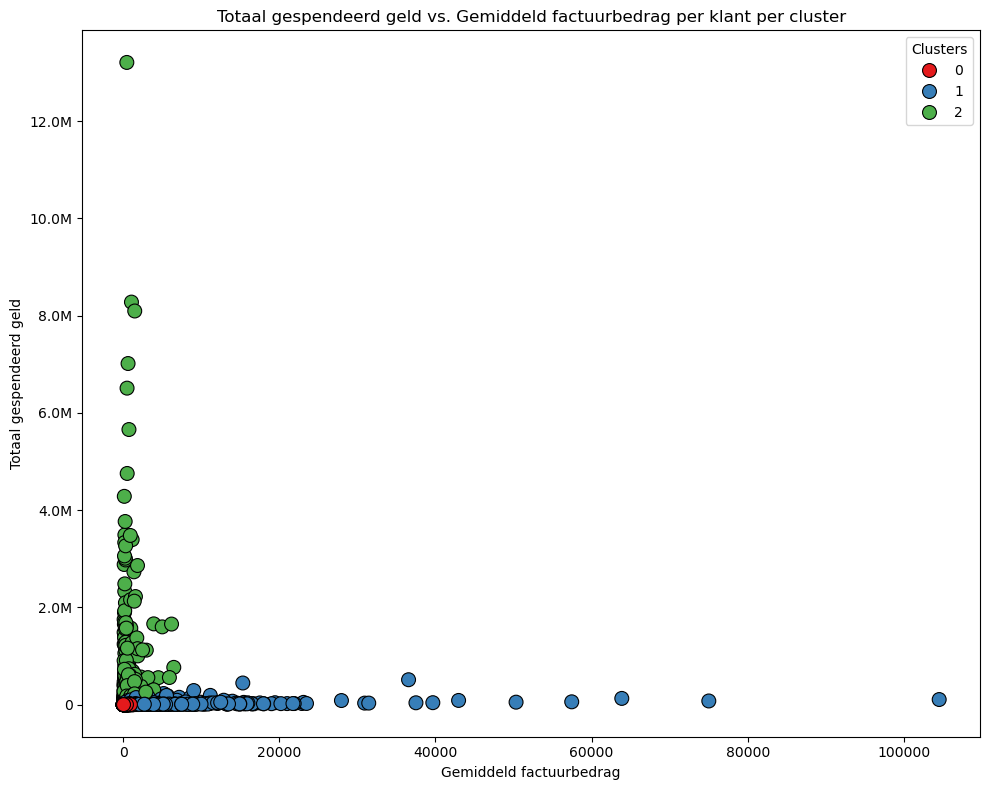
\includegraphics[width=0.8\linewidth]{images/GMM/Analyse2GMM}
    \caption{Analyse van gemiddelde factuurbedrag vs. totaal gespendeerd bedrag per klant (GMM)}
    \label{fig:Analyse_GMM}
\end{figure}

\subsection*{DBSCAN}

\begin{figure}[H]
    \centering
    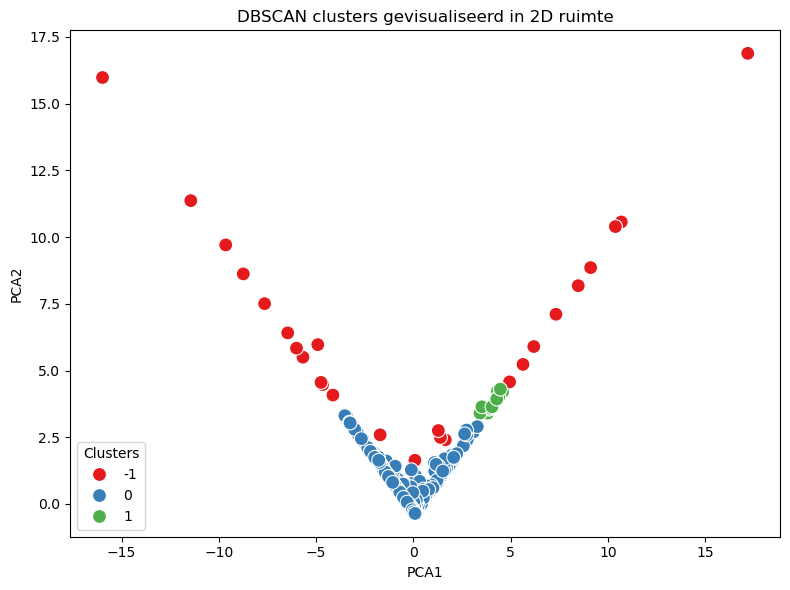
\includegraphics[width=0.8\linewidth]{images/DBSCAN/AnalyseDBSCAN}
    \caption{2D-representatie van de DBSCAN clusters met PCA}
    \label{fig:PCA_DBSCAN}
\end{figure}

\begin{figure}[H]
    \centering
    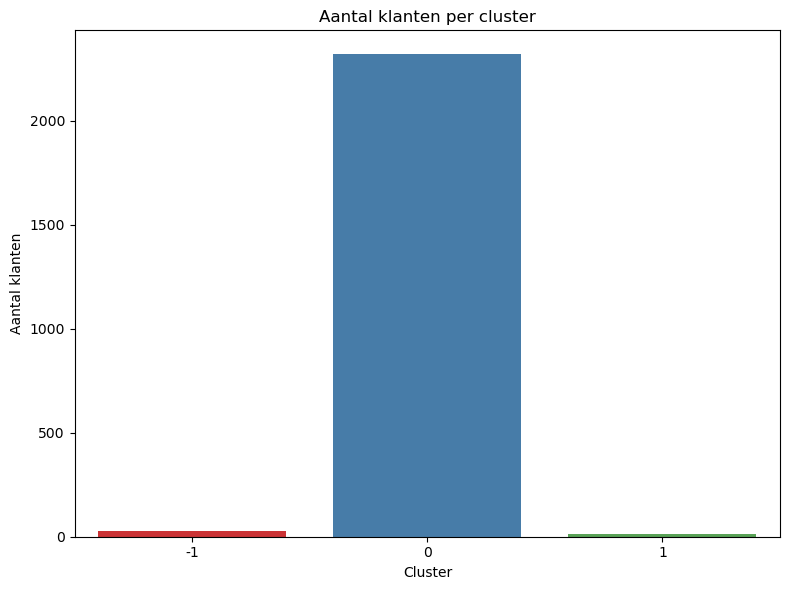
\includegraphics[width=0.8\linewidth]{images/DBSCAN/AantalKlantenDBSCAN}
    \caption{Aantal klanten per cluster (DBSCAN)}
    \label{fig:Klanten_DBSCAN}
\end{figure}

\begin{figure}[H]
    \centering
    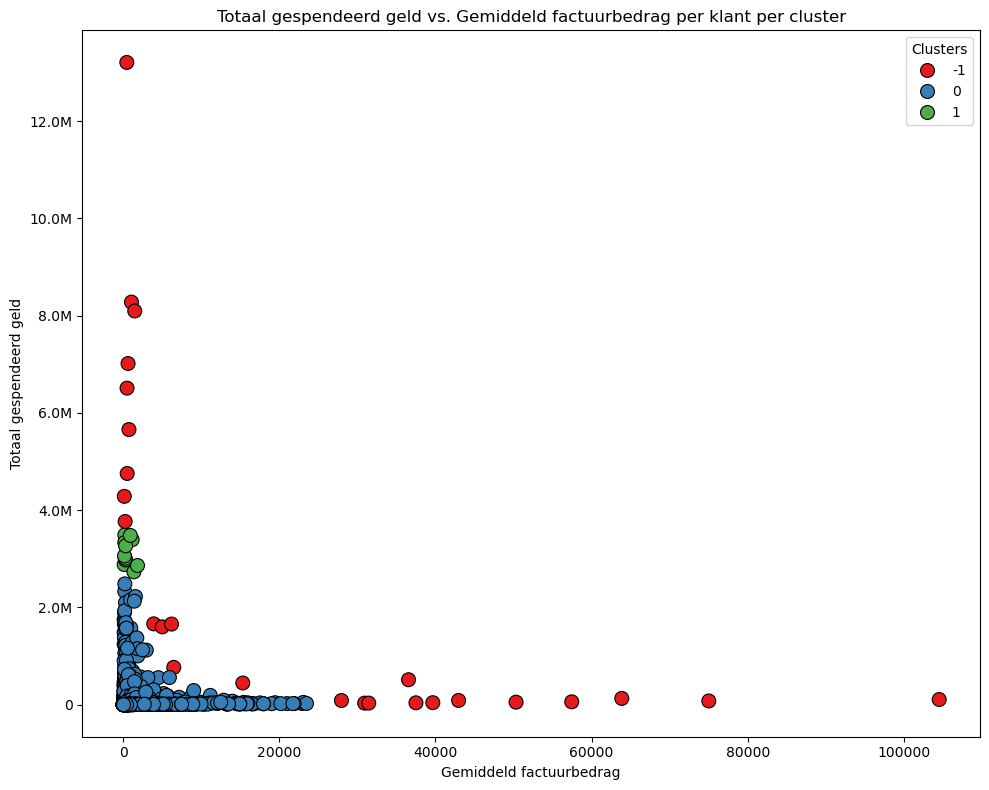
\includegraphics[width=0.8\linewidth]{images/DBSCAN/Analyse2DBSCAN}
    \caption{Analyse van gemiddelde factuurbedrag vs. totaal gespendeerd bedrag per klant (DBSCAN)}
    \label{fig:Analyse_DBSCAN}
\end{figure}


\subsection*{Categorisch segmentatiemodel}

Voor de categorische data kunnen de clusters niet altijd op dezelfde manier worden geanalyseerd als bij de numerieke segmentatiemodellen. Daarom wordt er gebruik gemaakt van andere grafieken en tabellen om inzicht te krijgen in de verdeling van klanten binnen de clusters.

\vspace{1em}

De eerste grafiek toont het aantal klanten per cluster, waarbij de x-as de clusters weergeeft en de y-as het aantal klanten per cluster. Deze grafiek biedt inzicht in hoe de klanten verdeeld zijn over de verschillende clusters.

\vspace{1em}

Naast de grafiek, wordt er ook een tabel gepresenteerd die de meest voorkomende waarden voor elk categorisch kenmerk binnen elk cluster weergeeft. Dit biedt een gedetailleerder overzicht van de segmentatie, waarbij de meest representatieve klantkenmerken voor elk cluster worden getoond. De tabel bevat bijvoorbeeld de meest voorkomende klantgroep, activiteit, competentiecentrum en producttype per cluster. Dit helpt bij het begrijpen van de klantprofielen die zich in de verschillende segmenten bevinden.


\begin{figure}[H]
    \centering
    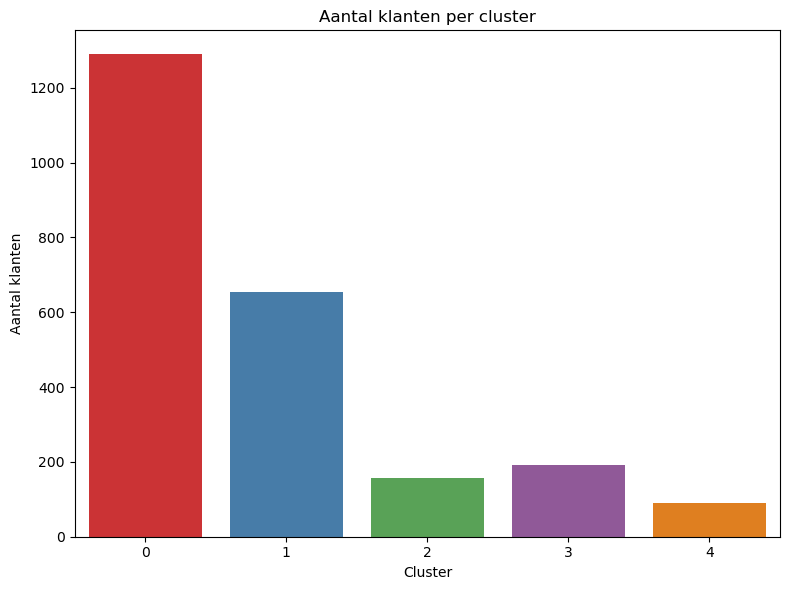
\includegraphics[width=1\linewidth]{images/Kmodes/AantalKlantenCluster}
    \caption{Aantal klanten per cluster (K-Modes))}
    \label{fig:KlantenK-Modes}
\end{figure}


\begin{table}[H]
    \centering
    \begin{tabular}{|c|c|c|c|c|c|}
        \hline
        \textbf{Cluster} & \textbf{Klantgroep} & \textbf{Activiteit} & \textbf{Competentiecentrum} & \textbf{Producttype} & \textbf{Aantal Klanten} \\
        \hline
        0 & Overige & Trading & Unknown & Unknown & 1289 \\
        1 & Utiliteit & Trading & Thermal insulation & Board / sheets & 653 \\
        2 & Installateur & Trading & Accessories & Unknown & 90 \\
        3 & Utiliteit & Trading & Acoustic insulation & Unknown & 193 \\
        4 & OEM & Trading & Thermal insulation & Unknown & 158 \\
        \hline
    \end{tabular}
    \caption{Aantal klanten per cluster op basis van K-Modes centroiden}
    \label{tab:AantalKlantenPerClusterCategorie}
\end{table}

\subsection{Conclussie}

De uiteindelijke beoordeling van de effectiviteit van de segmentatiemodellen wordt in de volgende fase uitgevoerd, wanneer de invloed van de segmentatie op de nauwkeurigheid van het regressiemodel kan worden geanalyseerd. In deze fase worden de trends van elk model kort besproken.

\subsection*{K-Means}

Met K-Means is er een duidelijk patroon te herkennen. Groep 0 bevat de grootste hoeveelheid klanten en kan worden beschouwd als de algemene groep. Groep 1 omvat klanten met een hoog gemiddeld factuurbedrag, maar een lage totaal besteding. Ten slotte bevat groep 2 klanten met een laag gemiddeld factuurbedrag, maar een hoge totale besteding.


\subsection*{GMM}

Bij GMM zijn er vergelijkbare patronen als bij K-Means. Groep 0 bevat klanten met zowel een laag totaal besteed bedrag als een laag gemiddeld factuurbedrag. Groep 1 omvat klanten met een hoog gemiddeld factuurbedrag en een laag totaal besteed bedrag. Ten slotte heeft groep 2 klanten met een hoog totaal besteed bedrag, maar een laag gemiddeld factuurbedrag. Wat opvalt bij GMM is dat de groepen minder geneigd zijn om alleen de outliers te bevatten, maar in plaats daarvan meer klanten opnemen, waardoor elke groep breder vertegenwoordigd is.

\subsection*{DBSCAN}

Bij DBScan is het anders. Er is één algemene groep, groep 0, die een grote hoeveelheid klanten bevat. Deze groep vertoont veel variatie in zowel het totaal besteed bedrag als het gemiddelde factuurbedrag, wat betekent dat zowel klanten met lage als hoge bestedingen en factuurbedragen in deze groep vallen. Vervolgens is er groep 1, die klanten omvat die tussen de 3 miljoen en 3,75 miljoen hebben besteed, met een laag gemiddeld factuurbedrag. Ten slotte zijn er de outliers volgens DBScan, die als groep -1 worden geclassificeerd. Deze klanten hebben aan de ene kant een hoge totaal besteed bedrag en een laag gemiddeld factuurbedrag, terwijl aan de andere kant klanten met een hoog gemiddeld factuurbedrag en een laag totaal besteed bedrag vallen. Daarnaast zijn er ook enkele klanten die een beetje buiten de algemene groep vallen.

\newpage

\subsection*{K-Modes}

Bij K-Modes clustering zijn vijf klantgroepen gevormd op basis van categorische kenmerken zoals klantgroep, activiteit, competentiecentrum en producttype. Het aantal clusters is vooraf bepaald op vijf.

\vspace{1em}

Groep 0 is de grootste en bestaat voornamelijk uit klanten die onder "Overige" vallen. Bij veel van deze klanten zijn de gegevens over het competentiecentrum en producttype niet bekend. Het lijkt vooral een restgroep te zijn voor klanten die moeilijk in een andere groep te plaatsen zijn of waarvan de gegevens onvolledig zijn.

\vspace{1em}

Groep 1 bestaat vooral uit klanten in de klantgroep "Utiliteit", die zich richten op thermische isolatie. Zij kopen vooral producten uit de categorie "Board / sheets". Deze groep heeft een duidelijk profiel en is goed te onderscheiden van de andere groepen.

\vspace{1em}

Groep 2 is de kleinste groep en bestaat voornamelijk uit "Installateurs", die vooral accessoires als competentie centrum hebben. De beperkte grootte van deze groep wijst erop dat het om een meer gespecialiseerde niche gaat binnen de klantengroep.

\vspace{1em}

Groep 3 bevat opnieuw klanten uit de "Utiliteit", maar in dit geval richten ze zich op akoestische isolatie. Dit laat zien dat er binnen dezelfde klantgroep duidelijke verschillen zijn in voorkeur en focus, zoals het onderscheid tussen thermische en akoestische isolatie.

\vspace{1em}

Groep 4 bestaat uit OEM-klanten, die ook actief zijn in thermische isolatie. Het producttype is bij deze groep vaak onbekend, maar ze vormen een aparte groep met een eigen profiel, dat vooral bepaald wordt door hun klanttype.

\vspace{1em}

De verdeling van de klanten over deze clusters en hun specifieke kenmerken zijn te zien in Tabel~\ref{tab:AantalKlantenPerClusterCategorie}.

\newpage

\section{Regressiemodellen met klantsegmentatie}

In deze fase van de Proof of Concept (POC) wordt een combinatie gemaakt van de regressiemodellen uit Fase 3 en de segmentatiemodellen uit Fase 4. Het doel is om te analyseren welk regressiemodel het meest verbetert door de klantsegmentatie. Elk regressiemodel dat in Fase 3 is ontwikkeld, wordt gecombineerd met de segmentatiemodellen die in Fase 4 zijn gemaakt, en de prestaties van de modellen worden vervolgens geëvalueerd.

\subsection{Code en Implementatie}

Voor de implementatie van de regressiemodellen met klantsegmentatie is dezelfde code en dezelfde imports gebruikt als in Fase 3. Het enige verschil is dat de clusters, die uit de segmentatiemodellen in Fase 4 komen, aan de dataset zijn toegevoegd. Dit wordt gedaan door de klantsegmentatie per maand te koppelen aan de regressievoorspellingen.

\vspace{1em}

In plaats van enkel de turnover per jaar-maand te voorspellen, wordt de turnover nu gesplitst per cluster binnen dezelfde jaar-maand. Voor iedere maand wordt de turnover per cluster voorspeld. Vervolgens worden de voorspellingen per cluster gecombineerd om de uiteindelijke voorspellingen per maand te verkrijgen. Dit maakt het mogelijk om de prestaties van het model per cluster te evalueren en de MSE, MAE en RMSE te vergelijken, zoals te zien is in Tabel~\ref{tab:model_evaluation}, zodat geanalyseerd kan worden in hoeverre klantsegmentatie de voorspellingen verbetert.

\vspace{1em}

Voor K-Means werd ervoor gekozen om zowel de resultaten met drie clusters als met twee clusters te evalueren. De motivatie hiervoor is dat bij het gebruik van drie clusters, groep 1 zeer weinig datapunten bevatte. Dit werd ondervonden tijdens het programmeren van de combinatie van Linear Regression en K-Means, toen de maatstaven onverwacht hoog terugkwamen. Het bleek dat K-Means met drie clusters niet optimaal was voor het bereiken van nauwkeurige voorspellingen.

In de aangepaste versie werden de datapunten uit de inconsistente cluster samengevoegd met de grootste cluster.

\subsection{Resultaten}

In deze sectie worden de resultaten gepresenteerd voor alle regressiemodellen in combinatie met de verschillende segmentatiemodellen. De prestaties worden geëvalueerd aan de hand van drie standaardcriteria: MAE, RMSE en MSE. Daarbij wordt een overzichtstabel opgesteld met de segmentatiemodellen per regressiemodel. Daarnaast wordt per segmentatiemodel een grafiek getoond die de voorspelde en de werkelijke omzet met elkaar vergelijkt.


\subsection*{Lineaire Regressie}

Uit de evaluatie van de lineaire regressie in combinatie met de verschillende segmentatiemodellen blijkt dat geen enkel segmentatiemodel een positief effect heeft op de prestaties. Alleen K-Means met twee clusters komt dicht bij het oorspronkelijke model, maar dit resulteert nog steeds niet in een verbetering van de modelprestaties.

\vspace{1em}

Hieruit kunnen we dus concluderen dat lineaire regressie geen verbeteringen oplevert voor de precisie van het model in combinatie met de segmentatiemodellen.

\begin{table}[H]
    \centering
    \caption{Evaluatie van Segmentatiemodellen (Lineare Regressie)}
    \label{tab:segmentation_model_evaluation}
    \begin{tabular}{|l|r|r|r|}
        \hline
        \textbf{Segmentatiemodel} & \textbf{MSE} & \textbf{RMSE} & \textbf{MAE} \\ \hline
        Geen Segmentatie         & 202,982,205,716 & 450,535 & 346,951  \\ \hline
        DBSCAN                   & 203,660,022,011 & 451,287 & 366,047 \\ \hline
        GMM                      & 213,496,413,842 & 462,057 & 359,523 \\ \hline
        K-Means                  & 1,564,135,315,178 & 1,250,654 & 1,105,220 \\ \hline
        K-Means (2 clusters)     & 202,987,515,188 & 450,541 & 346,944 \\ \hline
        K-Modes                  & 235,814,056,435 & 485,607 & 375,252 \\ \hline
    \end{tabular}
\end{table}

\subsection*{Random Forest}

Met Random Forest zien we een duidelijke verbetering bij het gebruik van elk segmentatiemodel in vergelijking met het model zonder segmentatie. De twee beste segmentatiemodellen zijn GMM en K-Means (2 clusters), die beide beter presteren dan de andere modellen. Het valt op dat de MAE voor GMM lager is dan voor K-Means (2 clusters), wat betekent dat er minder kleine afwijkingen zijn in de voorspellingen. Aan de andere kant heeft K-Means (2 clusters) een lagere RMSE, wat erop wijst dat de voorspellingen dichter bij de werkelijke waarden liggen, met minder extreme afwijkingen.



\begin{table}[H]
    \centering
    \caption{Evaluatie van Segmentatiemodellen (Random Forest}
    \label{tab:rf_segmentation_model_evaluation}
    \begin{tabular}{|l|r|r|r|}
        \hline
        \textbf{Segmentatiemodel} & \textbf{MSE} & \textbf{RMSE} & \textbf{MAE} \\ \hline
        Geen Segmentatie         & 242,022,929,294 & 491,598 & 378,430 \\ \hline
        DBSCAN                   & 195,606,503,305 & 442,274 & 354,030 \\ \hline
        GMM                      & 181,570,304,039 & 426,111 & 323,223 \\ \hline
        K-Means                  & 191,538,053,557 & 437,651 & 348,390 \\ \hline
        K-Means (2 clusters)     & 173,878,934,037 & 416,988 & 331,119 \\ \hline
        K-Modes                  & 197,406,370,649 & 444,304 & 342,233 \\ \hline
    \end{tabular}
\end{table}

\subsection*{XGBoost}

Met XGBoost zien we een verbetering bij het gebruik van elk segmentatiemodel in vergelijking met het model zonder segmentatie. De twee segmentatiemodellen die het beste presteren zijn DBSCAN en GMM. DBSCAN heeft een lagere RMSE, wat aangeeft dat het model minder zware uitbijters bevat, terwijl GMM een lagere MAE heeft, wat duidt op minder kleine afwijkingen in de voorspellingen. 

\begin{table}[H]
    \centering
    \caption{Evaluatie van Segmentatiemodellen (XGBoost)}
    \label{tab:segmentation_model_evaluation_xgboost}
    \begin{tabular}{|l|r|r|r|}
        \hline
        \textbf{Segmentatiemodel} & \textbf{MSE} & \textbf{RMSE} & \textbf{MAE} \\ \hline
        Geen Segmentatie         & 282,605,525,485 & 531,607 & 376,649 \\ \hline
        DBSCAN                   & 198,351,735,089 & 445,367 & 331,881 \\ \hline
        GMM                      & 212,792,775,817 & 461,295 & 328,150 \\ \hline
        K-Means                  & 201,899,764,153 & 449,333 & 342,673 \\ \hline
        K-Means (2 clusters)     & 222,381,530,790 & 471,573 & 369,660 \\ \hline
        K-Modes                  & 219,390,746,160 & 468,392 & 359,734 \\ \hline
    \end{tabular}
\end{table}


\subsection*{Conclusie}

Zonder segmentatie was het beste model lineaire regressie. Dit was ook het enige regressiemodel dat geen verbeteringen zag met het gebruik van segmentatie. Na het integreren van segmentatie presteerden alle XGBoost en Random Forest-modellen beter dan het lineaire regressiemodel zonder segmentatie.

\vspace{1em}

De beste combinatie hierin was Random Forest met K-Means (2 clusters) voor RMSE en MSE, en Random Forest met GMM voor MAE. Deze bevinding toont aan dat segmentatie in combinatie met de juiste modelkeuze leidt tot verbeterde prestaties.

\newpage

\subsection{Resultaten Segmentatiemodellen}

In deze sectie worden de prestaties van de verschillende segmentatiemodellen geëvalueerd in combinatie met de regressiemodellen, buiten lineaire regressie aangezien hier geen enkele verbetering is opgetreden door de segmentatie. De impact van de segmentatie op de modelnauwkeurigheid wordt geanalyseerd aan de hand van de maatstaven. Elk segmentatiemodel wordt afzonderlijk beoordeeld om te begrijpen hoe de segmentatie de prestaties van de regressiemodellen beïnvloedt.


\subsection*{DBScan}

DBSCAN toont bij beide regressiemodellen een duidelijke verbetering in de maatstaven vergeleken met het model zonder segmentatie. In combinatie met XGBoost levert DBSCAN de beste resultaten voor zowel RMSE als MSE, en het tweede beste resultaat voor MAE. Echter, bij het gebruik van het Random Forest-model behaalt DBSCAN de voorlaatste positie, achter K-Means voor zowel RMSE als MSE, en behaalt het de hoogste MAE.

\vspace{1em}

Hieruit kan afgeleid worden dat DBSCAN goed samenwerkt met XGBoost maar niet met Random Forest.

\subsection*{GMM}

GMM toont bij beide regressiemodellen een duidelijke verbetering in de maatstaven vergeleken met het model zonder segmentatie. Bij Random Forest behaalt GMM de beste MAE en de tweede beste RMSE en MSE. Bij XGBoost levert GMM opnieuw de beste MAE, maar behaalt het de derde plaats voor zowel RMSE als MSE.

\vspace{1em}

Hieruit kan worden afgeleid dat GMM effectief is in het verminderen van kleine fouten, maar niet het beste model is om zware uitbijters te verkleinen. Daarnaast blijkt GMM goed samen te werken met zowel XGBoost als Random Forest.

\newpage

\subsection*{K-Means}

Voor K-Means en K-means (2 clusters) zien we een duidelijke verbetering in de maatstaven vergeleken met het model zonder segmentatie.

\subsubsection*{K-Means}

Bij Random Forest is de verbetering voor K-Means minder significant in vergelijking met de andere modellen, met de derde hoogste MSE en RMSE, en de op één na hoogste MAE. Bij XGBoost presteert K-Means beter, waar het de tweede beste RMSE en MSE oplevert, en het derde beste MAE.

\vspace{1em}

Hieruit kan worden geconcludeerd dat K-Means beter presteert in combinatie met XGBoost dan met Random Forest. Hoewel K-Means in beide gevallen beter scoort dan het model zonder segmentatie, hoort het over het algemeen niet bij de sterkste segmentatiemodellen in deze analyse.


\subsubsection*{K-Means (2 clusters)}

K-Means (2 clusters) behaalt de beste RMSE en MSE in combinatie met Random Forest en scoort daar ook de tweede beste MAE. In combinatie met XGBoost zijn de resultaten echter aanzienlijk minder, met de slechtste RMSE en MAE van alle segmentatiemodellen.

\vspace{1em}

Hieruit kunnen we concluderen dat K-Means (2 clusters) vooral goed presteert in combinatie met Random Forest, maar duidelijk minder effectief is in combinatie met XGBoost.


\subsection*{K-Modes}

Voor K-Modes zien we een duidelijke verbetering in de maatstaven vergeleken met het model zonder segmentatie. Met Random Forest heeft K-Modes de hoogste RMSE en MSE en de derde hoogste MAE, terwijl het bij XGBoost de tweede slechtste RMSE en tweede slechtste MAE behaalt.

\vspace{1em}

Hieruit kan besloten worden dat K-Modes, als enig categorisch segmentatiemodel, minder goed presteerde in vergelijking met de andere segmentatiemodellen.

\newpage

\subsection*{Conclusie}


Gezien het gebruik van twee verschillende regressiemodellen, Random Forest en XGBoost, zijn aparte rangschikkingen opgesteld om de beste segmentatiemodellen te evalueren. De rangschikkingen zijn opgesplitst op basis van de twee maatstaven: RMSE en MAE. Deze splitsing is noodzakelijk omdat de keuze tussen deze twee afhankelijk is van de specifieke doelstellingen van het model. RMSE is gevoeliger voor grotere afwijkingen en is nuttig wanneer het minimaliseren van deze van belang is. MAE daarentegen biedt een meer gebalanceerde benadering, waarbij de gemiddelde afwijking per voorspelling wordt benadrukt, wat geschikt is voor situaties waarin kleinere afwijkingen belangrijker zijn.

\vspace{1em}

Uit de resultaten blijkt dat, voor het minimaliseren van grote afwijkingen, K-Means (2 clusters) het beste presteert voor Random Forest, terwijl DBSCAN het beste presteert voor XGBoost. Voor het minimaliseren van kleinere afwijkingen blijkt het GMM-model de beste keuze te zijn voor zowel Random Forest als XGBoost.



\begin{table}[H]
    \centering
    \caption{Evaluatie van segmentatiemodellen (Random Forest) - Rangschikking op RMSE en MAE}
    \label{tab:rf_segmentation_model_evaluation_combined}
    \begin{tabular}{|l|l|r|l|r|}
        \hline
        \textbf{Rang} & \textbf{Model (RMSE)} & \textbf{RMSE} & \textbf{Model (MAE)} & \textbf{MAE} \\ \hline
        1 & K-Means (2 clusters)     & 416,988 & GMM                      & 323,223 \\ \hline
        2 & GMM                      & 426,111 & K-Means (2 clusters)     & 331,119 \\ \hline
        3 & K-Means                  & 437,651 & K-Modes                  & 342,233 \\ \hline
        4 & DBSCAN                   & 442,274 & K-Means                  & 348,390 \\ \hline
        5 & K-Modes                  & 444,304 & DBSCAN                   & 354,030 \\ \hline
        6 & Geen Segmentatie         & 491,598 & Geen Segmentatie         & 378,430 \\ \hline
    \end{tabular}
\end{table}

\begin{table}[H]
    \centering
    \caption{Evaluatie van segmentatiemodellen (XGBoost) - Rangschikking op RMSE en MAE}
    \label{tab:segmentation_model_evaluation_xgboost_combined}
    \begin{tabular}{|l|l|r|l|r|}
        \hline
        \textbf{Rang} & \textbf{Model (RMSE)} & \textbf{RMSE} & \textbf{Model (MAE)} & \textbf{MAE} \\ \hline
        1 & DBSCAN                   & 445,367 & GMM                      & 328,150 \\ \hline
        2 & K-Means                  & 449,333 & DBSCAN                   & 331,881 \\ \hline
        3 & GMM                      & 461,295 & K-Means                  & 342,673 \\ \hline
        4 & K-Modes                  & 468,392 & K-Modes                  & 359,734 \\ \hline
        5 & K-Means (2 clusters)     & 471,573 & K-Means (2 clusters)     & 369,660 \\ \hline
        6 & Geen Segmentatie         & 531,607 & Geen Segmentatie         & 376,649 \\ \hline
    \end{tabular}
\end{table}





% Voeg hier je eigen hoofdstukken toe die de ``corpus'' van je bachelorproef
% vormen. De structuur en titels hangen af van je eigen onderzoek. Je kan bv.
% elke fase in je onderzoek in een apart hoofdstuk bespreken.

%\input{...}
%\input{...}
%...

%%=============================================================================
%% Conclusie
%%=============================================================================

\chapter{Conclusie}%
\label{ch:conclusie}

% TODO: Trek een duidelijke conclusie, in de vorm van een antwoord op de
% onderzoeksvra(a)g(en). Wat was jouw bijdrage aan het onderzoeksdomein en
% hoe biedt dit meerwaarde aan het vakgebied/doelgroep? 
% Reflecteer kritisch over het resultaat. In Engelse teksten wordt deze sectie
% ``Discussion'' genoemd. Had je deze uitkomst verwacht? Zijn er zaken die nog
% niet duidelijk zijn?
% Heeft het onderzoek geleid tot nieuwe vragen die uitnodigen tot verder 
%onderzoek?

In dit onderzoek is de onderzoeksvraag "Hoe kan klantsegmentatie op basis van aankoopgedrag de nauwkeurigheid van salesvoorspellingen verbeteren?" beantwoord aan de hand van een proof-of-concept.

\vspace{1 em}

Dit onderzoek en de uitgewerkte proof-of-concepts vormen de basis voor het inzetten van salesvoorspellingen binnen IPCOM NV. Door klantsegmentatie te combineren met regressiemodellen worden nauwkeurigere voorspellingen mogelijk gemaakt, wat financiële managers ondersteunt bij het plannen van budgetten en het nemen van strategische beslissingen.

\vspace{1 em}

Allereerst werd in de fase \textit{Salesvoorspellingsmodellen} van de proof-of-concept een werden enkele regressiemodellen uitgewerkt, waaronder lineaire regressie, Random Forest en XGBoost, evenals het forecastmodel SARIMA. Deze modellen werden met elkaar vergeleken om de volgende deelvragen te beantwoorden:

\begin{itemize}
    \item Wat is efficiënter bij het voorspellen van sales, forecastmethoden zoals SARIMA of regressiemodellen?
    \item Welke regressiemodellen presteren het best bij het voorspellen van sales?
\end{itemize}

\vspace{1 em}

Uit de resultaten bleek dat SARIMA in deze context het slechtst presterende model was. Daarom kan worden geconcludeerd dat regressiemodellen hier efficiënter zijn, op basis van precisie.

\vspace{1 em}

Daarnaast blijkt uit de vergelijking van alle regressiemodellen kon ook worden geconcludeerd dat zonder klantsegmentatie het lineaire regressiemodel het beste presteerde, gebaseerd op de maatstaven RMSE, MSE en MAE, vergeleken met XGBoost en Random Forest.

\vspace{1 em} 

Ten slotte werden alle regressiemodellen gecombineerd met de klantsegmentatie uit fase \textit{Klantsegmentatie} van de proof-of-concept. Hiermee konden de volgende deelvragen worden beantwoord:

\begin{itemize}
    \item Hoe kan klantsegmentatie effectief worden geïntegreerd in een regressiemodel voor salesvoorspellingen om de nauwkeurigheid te verbeteren?
    \item Welke clusteringtechnieken, zoals K-means, GMM, DBSCAN en K-Modes, leveren de meest betekenisvolle klantsegmenten op voor het verbeteren van salesvoorspellingen?
    \item Welke regressiemodellen presteren het best bij het voorspellen van sales in combinatie met klantsegmentatie?
\end{itemize}

Tijdens het uitvoeren van \textit{Regressiemodellen met klantsegmentatie} werd de meest effectieve manier gevonden om klantsegmentatie te integreren in de regressiemodellen. Dit gebeurde door elk cluster aan de bijbehorende klanten toe te wijzen en bij het samenbrengen van de maandelijkse data de splitsing per cluster te behouden. Op deze manier werd er per cluster en per maand een voorspelling gemaakt.

\vspace{1 em} 

Op basis van de resultaten van alle gecombineerde modellen bleek dat GMM over het algemeen de beste prestaties leverde voor zowel Random Forest als XGBoost. K-means (2 clusters) leverde in combinatie met Random Forest het beste resultaat op, maar was tegelijkertijd het slechtste segmentatiemodel in combinatie met XGBoost. K-means presteerde gemiddeld bij beide modellen, terwijl DBSCAN voor XGBoost het beste segmentatiemodel was, maar minder goed presteerde in combinatie met Random Forest.

\vspace{1 em} 

Hierdoor is het moeilijk om eenduidig te bepalen welk klantsegmentatiemodel het beste is. Wel kan worden gesteld dat K-means (2 clusters) het beste presterende gecombineerde model opleverde, terwijl GMM de beste algemene prestaties behaalde over beide regressiemodellen, Random Forest en XGBoost. Het slechtste model is duidelijk aan te wijzen, aangezien K-modes, hoewel het in beide modellen enige verbetering liet zien ten opzichte van geen segmentatie, duidelijk minder goed presteerde dan de andere klantsegmentatiemodellen.


\vspace{1 em} 

Daarnaast was het best presterende regressiemodel in combinatie met klantsegmentatie het Random Forest-model. Dit model presteerde met elk segmentatiemodel beter dan het beste regressiemodel zonder segmentatie op basis van RMSE. Dit toont aan dat Random Forest het meeste voordeel haalt uit klantsegmentatie. 

\vspace{1 em} 

Bij XGBoost presteerden alle modellen beter met klantsegmentatie, maar slechts twee modellen deden het beter dan het beste regressiemodel zonder segmentatie op basis van RMSE. Dit toont aan dat XGBoost wel voordeel haalt uit klantsegmentatie maar niet zoveel vergeleken met Random Forest.

\vspace{1 em} 

Daarnaast liet het lineaire regressiemodel, dat vóór de integratie van klantsegmentatie het nauwkeurigst presteerde, geen enkele verbetering zien door het gebruik van klantsegmentatie. Hieruit kunnen we concluderen dat lineaire regressie geen voordeel haalt uit de segmentatie van klanten.

\vspace{1 em} 

Ten slotte is de onderzoeksvraag "Kan klantsegmentatie op basis van aankoopgedrag de nauwkeurigheid van salesvoorspellingen verbeteren?" beantwoord. Uit de resultaten van de laatste fase van het proof-of-concept blijkt dat het gebruik van klantsegmentatie duidelijke verbeteringen oplevert. Het beste resultaat werd behaald met het Random Forest-model in combinatie met K-means (2 clusters).

\vspace{1 em} 

Dit onderzoek had op bepaalde vlakken nog verder verbeterd kunnen worden, bijvoorbeeld door technieken zoals quantization en andere optimalisaties toe te voegen. Deze zijn echter niet meegenomen, omdat de focus lag op het bewijzen van de onderzoeksvraag. In de context van IPCOM NV kunnen deze verbeteringen in een volgende fase alsnog worden geïmplementeerd.




%---------- Bijlagen -----------------------------------------------------------

\appendix

\chapter{Onderzoeksvoorstel}

Het onderwerp van deze bachelorproef is gebaseerd op een onderzoeksvoorstel dat vooraf werd beoordeeld door de promotor. Dat voorstel is opgenomen in deze bijlage.

%% TODO: 
%\section*{Samenvatting}

% Kopieer en plak hier de samenvatting (abstract) van je onderzoeksvoorstel.
Dit onderzoek gaat na of het gebruik van klantsegmentatie op basis van hun koopgedrag de nauwkeurigheid van een regressievoorspellingsmodel kan verbeteren. Een uitgebreid plan werd uitgevoerd en de resultaten hiervan werden geanalyseerd voor het bedrijf IPCOM NV. Dit werd onderzocht met behulp van de Microsoft Fabric-omgeving, en meer specifiek de Machine Learning-notebooks en Dataflows. Binnen deze omgeving werd historische salesdata op artikelniveau verzameld en geanalyseerd om klanten te groeperen op basis van hun aankoopgedrag, zoals patronen in hun uitgaves, aankoopfrequentie en product voorkeuren. Vervolgens werd dit gebruikt in regressiemodellen om te bepalen of de voorspelling meer of minder accuraat zijn met de klanten segmentatie. De resultaten zijn beoordeeld op basis van nauwkeurigheid van het model en dit werd gemeten door prestatie-indicators zoals de Mean Absolute Error (MAE) en de Root Mean Squared Error (RMSE). Uit de resultaten van het onderzoek blijkt dat de klantsegmentatie effectief een bijdrage heeft aan de precisie van de voorspellingen met behulp van een regressie model. Dit onderzoek biedt inzicht in hoe bedrijfsspecifieke klantendata optimaal benut kan worden voor verdere optimalisaties binnen Microsoft Fabric’s Machine Learning-tools. 

% Verwijzing naar het bestand met de inhoud van het onderzoeksvoorstel
%---------- Inleiding ---------------------------------------------------------

% TODO: Is dit voorstel gebaseerd op een paper van Research Methods die je
% vorig jaar hebt ingediend? Heb je daarbij eventueel samengewerkt met een
% andere student?
% Zo ja, haal dan de tekst hieronder uit commentaar en pas aan.

%\paragraph{Opmerking}

% Dit voorstel is gebaseerd op het onderzoeksvoorstel dat werd geschreven in het
% kader van het vak Research Methods dat ik (vorig/dit) academiejaar heb
% uitgewerkt (met medesturent VOORNAAM NAAM als mede-auteur).
% 

\section{Inleiding}%
\label{sec:inleiding}


Het voorspellen van sales en winst is een essentieel proces voor elk bedrijf dat strategische beslissingen wil nemen of financiële plannen wil opstellen. In de huidige tijd is het bijna onmogelijk om dit effectief te doen zonder gebruik te maken van data-analyse en andere technieken zoals klantsegmentatie. Bedrijven worden geconfronteerd met een steeds dynamischere markt, wat ervoor zorgt dat traditionele voorspellingsmethoden vaak tekortschieten. 

De doelgroep van dit onderzoek richt zich specifiek op managers en analisten in commerciële en financiële functies binnen bedrijven. Commercieel managers zijn verantwoordelijk voor het optimaliseren van verkoopstrategieën, terwijl financiële analisten gefocust zijn op het opstellen van nauwkeurige budgetten. Beide rollen zijn direct afhankelijk van betrouwbare en data gedreven voorspellingen om strategische beslissingen te ondersteunen.

Elk bedrijf wil de meest accurate voorspellingen om deze beslissingen op te baseren, maar de complexiteit van klantgedrag en marktveranderingen maakt dit steeds moeilijker. Traditionele voorspellingsmethoden schieten vaak tekort, omdat ze niet genoeg rekening houden met de dynamische behoeftes van klanten. Dit onderzoek richt zich op de vraag hoe het categoriseren van klanten op basis van hun aankoopgedrag de nauwkeurigheid van salesvoorspellingen kan verbeteren. Het doel is om inzicht te krijgen in hoe klantsegmentatie de precisie van voorspellingsmodellen kan verbeteren, zodat bedrijven beter geïnformeerde strategische keuzes kunnen maken.

In dit onderzoek worden verschillende deelvragen beantwoord.Ten eerste wordt onderzocht welke soorten klantdata het meest relevant zijn voor het begrijpen van koopgedrag en het voorspellen van toekomstige sales, aangezien deze data essentieel zijn voor het vormen van effectieve klantsegmenten. Daarnaast wordt gekeken naar welke methoden en technieken binnen Machine Learning en Python het beste kunnen worden toegepast om foutieve data te identificeren en te corrigeren tijdens de data-integratie, zodat betrouwbare input voor de voorspellingsmodellen wordt gegarandeerd. 

Vervolgens wordt onderzocht welke clusteringtechnieken, zoals K-means of hiërarchische clustering, de meest betekenisvolle klantsegmenten opleveren voor het verbeteren van salesvoorspellingen. Dit wordt aangevuld door de vraag welke regressiemodellen de beste prestaties leveren voor het voorspellen van sales. Tot slot wordt onderzocht welke methoden effectief kunnen worden toegepast om klantsegmentatie te integreren in een regressiemodel voor salesvoorspellingen, zodat het model de nauwkeurigheid van de voorspellingen verbetert.

Het eindresultaat van dit onderzoek is een proof-of-concept voor het bedrijf IPCOM NV, waarbij de nauwkeurigheid van salesvoorspellingen met en zonder klantsegmentatie wordt vergeleken. Het succes van deze bachelorproef wordt bepaald door het aantonen dat klantsegmentatie de precisie van de voorspellingen verbetert.

%---------- Stand van zaken ---------------------------------------------------

\section{Literatuurstudie}%
\label{sec:literatuurstudie}

Een vraag die veel managers zich stellen, is waarom het zo belangrijk is om sales en winst te voorspellen. Zoals beschreven in Sales Forecasting Management van \textcite{JohnT.Mentzer2004}, is het antwoord simpel: elke keer dat er een plan wordt gemaakt, wordt er impliciet ook een voorspelling gemaakt. Dit geldt voor zowel individuen als organisaties en vormt de basis voor strategisch plannen. Wanneer een organisatie financiële plannen maakt op basis van verwachte verkoopcijfers, helpt een nauwkeurige voorspelling om deze doelen realistisch en haalbaar te maken. Slechte voorspellingen leiden dan ook tot slechte financiële plannen.


Traditionele voorspellingsmethoden voor sales zijn vaak gebaseerd op tijdreeksen, dit betekent dat de vraag voor een product in het verleden kan gebruikt worden om de toekomstige vraag voor dit product te voorspellen. Deze methode werkt goed in markten waar de vraag stabiel blijft, maar kent beperkingen in meer dynamische markten. Het probleem is dat de vraag ook beïnvloed wordt door externe factoren zoals weersomstandigheden, economische ontwikkelingen, seizoensgebonden trends, consumentenvoorkeuren of zelfs veranderingen in het algemene sentiment. Tijdreeksen kunnen hier geen rekening mee houden, dit leidt tot minder nauwkeurige voorspellingen wanneer deze externe factoren groot zijn in belang. Een oplossing hiervoor zou een ander soort van voorspellingsmethoden zijn zoals causaal modelleren, met deze techniek kan je rekening houden met economische variabele, weersomstandigheden en marketingsstrategieën \autocite{UsugaCadavid2018}

In de literatuur worden verschillende soorten voorspellingen onderscheiden volgens \textcite{UsugaCadavid2018}, zoals vraagvoorspellingen (demand forecasting) en sales voorspellingen (sales forecasting). In dit onderzoek wordt de focus gelegd op sales voorspellingen. Sales voorspelling is gebaseerd op gegevens die direct zijn verzameld uit verkooppunten, zoals winkeltransacties. Deze gegevens zijn gevoelig voor invloeden zoals promoties of voorraadtekorten, waardoor sales voorspellingen vaak de effectiviteit van promoties en de beschikbaarheid van producten weerspiegelen, in plaats van de werkelijke vraag. Aan de andere kant richt vraagvoorspelling zich op het identificeren van de werkelijke marktvraag, waarbij de effecten van promoties en voorraadtekorten zijn gecorrigeerd. Het doel is om een nauwkeuriger beeld te krijgen van de vraag, onafhankelijk van tijdelijke invloeden zoals marketingcampagnes of voorraadbeheer. Dit verschil, hoewel subtiel, heeft een grote invloed op de de manier waarop voorspellingen worden gemaakt en hoe bedrijven hun supply chain kunnen afstemmen op de werkelijke marktvraag in plaats van alleen verkoopaantallen .

Big data biedt veel voordelen voor salesvoorspellingen, maar de integratie ervan is allesbehalve eenvoudig. \textcite{Boone2019} bespreken de strategische en praktische uitdagingen waarmee bedrijven worden geconfronteerd bij het incorporeren van big data in hun voorspellingsmodellen. Op strategisch niveau moet elk bedrijf beslissen of en hoeveel big data-technologieën ze willen integreren. Dit besluit hangt af van de potentiële voordelen van het gebruik van big data in vergelijking met de kosten van het verzamelen en analyseren van deze gegevens. 

Big data heeft het potentieel om productvoorspellingen te verbeteren en waardevolle inzichten te geven in klantgedrag. Echter, de praktische uitdaging van demand planners is de enorme hoeveelheid gegevens die verzameld wordt, zoals bijvoorbeeld de 2,5 petabytes aan data die Walmart elke uur verzamelt. De vraag die hierbij opkomt, is welke data bewaard moeten worden en hoe lang. 

Een belangrijk obstakel bij het gebruik van big data voor vraagvoorspellingen is de invloed van menselijke beoordelingen. Veel bedrijven baseren hun voorspellingen op "gevoel" en passen statistische modellen aan op basis van factoren die vraagvoorspellers moeilijk kunnen meten zoals marketingactiviteiten of seizoenstrends. Hoewel menselijke beoordeling de voorspellingen kan verbeteren, introduceert het vaak vooroordelen die de nauwkeurigheid verminderen. Boone et al. suggereren dat big data mogelijk de negatieve effecten van deze "aanpassingen" kan verminderen, maar ze erkennen dat de praktische integratie van big data in ERP-systemen veel uitdagingen met zich meebrengt





In een onderzoek uitgevoerd door \textcite{Neba2024}  op een Walmart-dataset werd ontdekt dat traditionele lineaire modellen vaak niet in staat zijn om de complexe, niet-lineaire relaties binnen retaildata vast te leggen. Deze modellen konden de ingewikkelde interacties tussen verschillende variabelen niet effectief begrijpen. Aan de andere kant toonden geavanceerdere ensemble-methoden, zoals Random Forest en Gradient Boosting Machines (GBM), aanzienlijk betere voorspellende nauwkeurigheid door de uitkomsten van meerdere besluitbomen te combineren. Deze methoden wisten verborgen patronen te identificeren en de voorspellingsprecisie te verbeteren.

Van de geavanceerde modellen bleek XGBoost het beste te presteren, met de laagste Mean Absolute Error (MAE) en Root Mean Squared Error (RMSE). Dit onderstreepte de superieure capaciteiten van XGBoost voor het maken van nauwkeurige verkoopvoorspellingen. De verbeterde prestaties werden toegeschreven aan de efficiënte implementatie van gradient boosting, evenals aan technieken zoals regularisatie en het omgaan met ontbrekende waarden, waardoor XGBoost het model van keuze werd voor accurate verkoopvoorspellingen.


Volgens Pareto’s 80/20-regel is een klein percentage van de klanten vaak verantwoordelijk voor een groot deel van de omzet van een bedrijf. Hoewel dit principe in veel gevallen wordt waargenomen, is het belangrijk om op te merken dat dit niet altijd strikt van toepassing is. Dit betekent dat het behouden van deze klanten enorm belangrijk en soms zelf belangrijker als nieuwe klanten aantrekken. \textcite{Wu2011} benadrukken in hun onderzoek naar klantsegmentatie het belang van het begrijpen van klantgedrag. Ze stellen at bedrijven effectieve marketingstrategieën te ontwikkelen op basis van klantsegmenten, waarbij ze de koopgewoonten van klanten analyseren. 

Een natuurlijk gevolg van klantsegmentatie is dat je klanten beter kunt bedienen door prijzen of aanbiedingen aan te passen aan hun individuele behoeften. Deze aanpak maakt het mogelijk voor bedrijven om prijzen of aanbiedingen af te stemmen op de specifieke kenmerken en behoeften van individuele klanten, in plaats van gebruik te maken van algemene en uniforme strategieën.

Een van de grootste voordelen van een gepersonaliseerde benadering is de positieve invloed op klantbehoud. Klanten die het gevoel hebben dat producten of diensten eerlijk en relevant zijn voor hun situatie, blijven loyaal aan het bedrijf. Daarnaast versterkt personalisatie het vertrouwen van klanten, doordat zij het gevoel krijgen als individu te worden behandeld in plaats van slechts een nummer in een database te zijn. Zo kunnen bijvoorbeeld trouwe klanten beloond worden met speciale aanbiedingen of kortingen, wat hun loyaliteit versterkt. Daarentegen kan een niet-gepersonaliseerde aanpak ervoor zorgen dat klanten zich niet gewaardeerd voelen of het idee krijgen dat ze te veel betalen. Dit vergroot de kans dat ze overstappen naar een concurrent, wat uiteindelijk kan resulteren in een hoger klantverloop.\autocite{Adeniran2024}


% Voor literatuurverwijzingen zijn er twee belangrijke commando's:
% \autocite{KEY} => (Auteur, jaartal) Gebruik dit als de naam van de auteur
%   geen onderdeel is van de zin.
% \textcite{KEY} => Auteur (jaartal)  Gebruik dit als de auteursnaam wel een
%   functie heeft in de zin (bv. ``Uit onderzoek door Doll & Hill (1954) bleek
%   ...'')


%---------- Methodologie ------------------------------------------------------

\section{Methodologie}%
\label{sec:methodologie}


\textbf{Fase 1: Data verzameling}

In deze fase wordt de benodigde data verzameld voor de klantsegmentatie en de salesvoorspellingen uit te voeren. De gegevens komen uit interne bronnen om een compleet overzicht van het klantgedrag en de verkoop te verkrijgen.

De focus ligt op het verzamelen van de verkoop- en artikeldata van Isopartner Nederland, een entiteit binnen IPCOM NV, aangezien deze data de meest accurate en betrouwbare bron vormt voor het opzetten van een proof of concept. De verzamelde data omvat transactiebedragen, marges, artikeldata, klant-ID en de datum van de  transactie. Het doel is om alle data dat een inzicht zou geven in het koopgedrag van de klant en voor het voorspellen van toekomstige sales te verzamelen. 

Daarnaast wordt er interne data verzameld die Isopartner Nederland momenteel niet heeft, namelijk gegevens over het aantal werkbare werkdagen per maand. Dit is van belang omdat het aantal werkdagen in een maand invloed kan hebben op de verkoopresultaten, bijvoorbeeld doordat langere maanden met meer werkdagen doorgaans tot hogere verkopen leiden. Deze gegevens zullen persoonlijk opgevraagd worden bij de contactpersonen binnen het bedrijf.

Op het einde van deze fase is alle nodige data verzameld en beschikbaar voor gebruik. Daarnaast wordt in deze fase de deelvraag beantwoord: "Welke soorten klantdata zijn het meest relevant voor het begrijpen van koopgedrag en het voorspellen van toekomstige sales?" Aangezien meeste data al beschikbaar is in de dataflows van Microsoft Fabric, wordt er voor deze fase 2 weken verwacht.


\textbf{Fase 2: Data-integratie en voorbereiding}

Nadat we alle data verzameld hebben in fase 1, worden de verschillende gegevensbronnen samengevoegd en voorbereid voor verdere analyses. Het doel is om een consistente dataset te creëren die gebruikt kan worden voor klantsegmentatie en salesvoorspellingen.

De verkoopdata, artikeldata, klantdata en de data over aantal werkdagen per maand worden samengebracht in één dataflow binnen de Microsoft Fabrics omgeving. Deze data wordt vervolgens opgeslagen en verder geoptimaliseerd in een datawarehouse binnen dezelfde Microsoft Fabric-omgeving.

Na het succesvol wegschrijven van de data, wordt er verder gewerkt aan het identificeren van potentiële foutieve data die niet gebruikt mag worden voor analyses. Dit omvat het opsporen van ontbrekende waarden, dubbele records of onjuiste gegevens. Hiervoor wordt gebruik gemaakt van Machine Learning Notebooks binnen Microsoft Fabric, waarbij Python Libraries zoals Panda’s worden toegepast om foutieve data te detecteren en aan te passen. 

Het eindproduct van deze fase zou een consistente dataset zijn, gereed voor verdere analyses en modellering. Ook wordt de deelvraag "Welke methoden en technieken binnen Machine Learning en Python kunnen het best worden gebruikt om foutieve data te identificeren en te corrigeren tijdens de data-integratie?" beantwoord. De geschatte tijdsduur voor deze fase is 1 week en 3 dagen.




\textbf{Fase 3: Klantsegmentatie en gedragspatronen analyse}

In deze fase ligt de focus op het uitvoeren van Exploratory Data Analysis (EDA) op de verzamelde data en het toepassen van clusteringtechnieken.  Het doel is het identificeren van welke variabelen het meest invloed hebben op de clustering en het opzetten van een volledig clusteringmodel. 

Tijdens de EDA worden de belangrijkste kenmerken van de data, zoals aankoopgedrag, productinformatie en werkbare werkdagen, grondig geanalyseerd met behulp van Pandas en Matplotlib. Dit helpt bij het bepalen van welke variabelen het meest bepalend zijn voor de clustering van de gegevens. Dit proces kan het identificeren van afwijkingen en correlaties tussen verschillende factoren vergemakkelijken.

Door clusteringalgoritmes zoals K-means of hiërarchische clustering toe te passen met behulp van Scikit-learn, worden de gegevens verdeeld in groepen die vergelijkbare eigenschappen vertonen. Daarna vergelijken we de resultaten van beide algoritmes om te bepalen welk model de meest betekenisvolle clusters oplevert. Dit gebeurt door de clusterresultaten te analyseren op basis van hun interne samenhang en de geschiktheid voor het gewenste resultaat, zoals het verbeteren van de nauwkeurigheid van salesvoorspellingen.

Het eindresultaat van deze fase is een geoptimaliseerd clusteringmodel dat klantsegmenten creëert op basis van hun aankoopgedrag, productinformatie en werkbare werkdagen. Dit model vormt de basis voor het verder verfijnen van salesvoorspellingen. In deze fase wordt tevens de deelvraag beantwoord: "Welke clusteringtechnieken, zoals K-means of hiërarchische clustering, leveren de meest betekenisvolle klantsegmenten op voor het verbeteren van salesvoorspellingen?" Voor deze fase wordt 3 weken verwacht.

\textbf{Fase 4: Salesvoorspellingen met regressiemodellen}

Het doel van deze fase is het ontwikkelen van een regressiemodel voor salesvoorspellingen zonder het gebruik van klantsegmentatie, zodat we later de prestaties van dit model kunnen vergelijken met het model dat klantsegmentatie bevat.

Dit wordt bereikt door verschillende regressiemodellen toe te passen, zoals lineaire regressie, decision tree-regressie en random forest-regressie, met behulp van de Python-libraries zoals scikit-learn. Elk model wordt geëvalueerd op basis van hun prestaties, met als belangrijkste metrics de Mean Squared Error (MSE) en Root Mean Squared Error (RMSE). De modellen worden getest door gebruik te maken van een train-test splits en cross-validatie, om ervoor te zorgen dat het gekozen model goed generaliseert naar nieuwe data en niet overfit. 

Het uiteindelijke resultaat van deze fase is het regressiemodel met de laagste MSE en RMSE, dat de basis zal vormen voor de volgende fase, waarin klantsegmentatie wordt geïntegreerd om de voorspellingen verder te verfijnen. De deelvraag die in deze fase beantwoord wordt is: "Welke regressiemodellen leveren de beste prestaties voor het voorspellen van sales?" Deze fase duurt 2 weken.

\textbf{Fase 5: Regressiemodel met klantsegmentatie en vergelijking}

In deze fase wordt het regressiemodel dat eerder is ontwikkeld verder verfijnd door de klantsegmentatie gegevens te integreren. Het doel is om te onderzoeken of het toevoegen van klantsegmentatie leidt tot verbeterde salesvoorspellingen. Dit wordt bereikt door de gegevens van de verschillende klantsegmenten, zoals koopgedrag en andere relevante kenmerken, te gebruiken om het regressiemodel te verbeteren. Het aangepaste model wordt vervolgens vergeleken met het eerdere model zonder klantsegmentatie aan de hand van de Mean Squared Error (MSE) en Root Mean Squared Error (RMSE) om te beoordelen of de segmentatie daadwerkelijk leidt tot een significante verbetering in de nauwkeurigheid van de salesvoorspellingen.

Het eindresultaat van deze fase is een regressiemodel dat de klantsegmentatiegegevens correct verwerkt. Dit zal bijdragen aan het beantwoorden van de hoofdonderzoeksvraag: 'Hoe kan klantsegmentatie de precisie van salesvoorspellingsmodellen verbeteren?' Bovendien wordt in deze fase de deelvraag beantwoord: 'Welke methoden kunnen worden toegepast om klantsegmentatie effectief te integreren in een regressiemodel voor salesvoorspellingen?' Deze fase duurt 2 weken.


%---------- Verwachte resultaten ----------------------------------------------
\section{Verwacht resultaat, conclusie}%
\label{sec:verwachte_resultaten}

In dit onderzoek wordt verwacht dat het toevoegen van klantsegmentatie aan het regressiemodel een significante verbetering zal opleveren in de nauwkeurigheid van de salesvoorspellingen. Het model met klantsegmentatie wordt verwacht lagere MSE- en RMSE-waarden te vertonen, wat duidt op een meer nauwkeurige voorspelling van de sales. Door klantsegmentatie toe te passen, wordt verondersteld dat de verschillende klantgroepen verschillende koopgedragingen vertonen, waardoor de voorspellingen beter afgestemd kunnen worden op specifieke klantgroepen. Dit zou moeten leiden tot een preciezere voorspelling van de verkoopresultaten.

De meerwaarde voor commerciële functies binnen bedrijven ligt in het beter begrijpen en bedienen van specifieke klantgroepen. Een model met klantsegmentatie kan helpen bij het ontwikkelen van gerichte marketingstrategieën. Dit verhoogt de efficiëntie van verkoopprocessen en kan leiden tot een groei in omzet, klanttevredenheid en mogelijk ook een verbetering van het aankoopbeheer.

Voor financiële functies biedt een model voor nauwkeurige salesvoorspellingen ondersteuning bij het maken van meer financiële beslissingen en budgetplanningen. Financiële analisten kunnen met behulp van deze voorspellingen beter inzicht krijgen in de inkomstenstromen, wat resulteert in verbeterde financiële stabiliteit en planning. Bovendien kunnen ook andere afdelingen, zoals HRM, hiervan profiteren bij het plannen van personeelsbehoeften.



%%---------- Andere bijlagen --------------------------------------------------
% TODO: Voeg hier eventuele andere bijlagen toe. Bv. als je deze BP voor de
% tweede keer indient, een overzicht van de verbeteringen t.o.v. het origineel.
%\input{...}

%%---------- Backmatter, referentielijst ---------------------------------------

\backmatter{}

\setlength\bibitemsep{2pt} %% Add Some space between the bibliograpy entries
\printbibliography[heading=bibintoc]

\end{document}
